\documentclass[11pt,a4paper]{article}

\usepackage[margin=2.3cm]{geometry}
\usepackage{amsmath,amssymb,amsthm}
\usepackage{booktabs}
\usepackage{graphicx}
\usepackage{hyperref}
\usepackage[sort&compress,numbers]{natbib}
\usepackage{caption,subcaption}
\usepackage{xcolor,colortbl}
\usepackage{array,longtable}
\usepackage{float}
\usepackage{rotating}

\definecolor{best}{rgb}{0,0.5,0}

\title{Generative and Adaptive Sampling Strategies for \\
       Neural Network Function Approximation in $L^2[0,1]$}
\author{}
\date{\today}

\begin{document}
\maketitle

\begin{abstract}
We compare \textbf{fifteen} sampling strategies for training a small neural
network to approximate diverse 1D test functions on $[0,1]$ under a
fixed sampling budget.  The strategies span fixed-grid (uniform,
Chebyshev, QMC), adaptive empirical (residual-based refinement),
generative (adversarial, normalising flow, MDN, diffusion / score
matching, importance sampling), particle-based (SVGD), uncertainty-based
(deep ensemble, GP-UCB), and policy-gradient (policy / meta-sampler)
approaches.  For each (function, algorithm) pair we record the
$L^2$ approximation error as a function of the number of sampling points,
revealing convergence rates and the point-allocation patterns that
drive them.
\end{abstract}

% ======================================================================
\section{Problem setting}
% ======================================================================
\label{sec:problem}

Let $f:[0,1]\to\mathbb{R}$ be a target function known only through
pointwise evaluations.  We are given a total budget $N$ of function
evaluations and a parametric approximator $u_\theta:[0,1]\to\mathbb{R}$
(here, a small MLP).  The goal is to choose evaluation locations
$\{x_i\}_{i=1}^N\subset[0,1]$ such that the $L^2$ error

\begin{equation}\label{eq:l2loss}
  \mathcal{L}(\theta) = \int_0^1 \bigl(u_\theta(x) - f(x)\bigr)^2\,dx
\end{equation}

is minimised.  The integral is estimated by trapezoidal quadrature on a
dense uniform grid $\{x_k^{\mathrm{ref}}\}_{k=1}^{N_{\mathrm{ref}}}$,
where $N_{\mathrm{ref}}$ is chosen individually per function to resolve
its finest features.

\subsection{Approximator architecture}

Unless otherwise noted, the approximator is a 4-hidden-layer MLP with
$[32,32,32,32]$ neurons and $\tanh$ activation ($\sim 3.2$K parameters).
It is deliberately small so that sampling quality dominates the error.
Alternative architectures (e.g., the MMNN with frozen random expansion
layers) can be supplied via the \texttt{--model} or
\texttt{--model-factory} API.

\subsection{Test-function library and downstream tasks}

The library contains 13 hand-crafted 1D functions plus a
programmatically-generated library of up to $200\times 3 = 600$
$L^2$-normalised functions partitioned into three classes:

\begin{itemize}
  \item \textbf{Smooth:} polynomials, trigonometric polynomials,
        rationals, exponentials --- slowly varying throughout $[0,1]$.
  \item \textbf{Oscillatory:} chirps, amplitude- and frequency-modulated
        sinusoids, multi-frequency superpositions --- high-frequency
        content everywhere.
  \item \textbf{Sharp:} Gaussian bumps, mollified steps, boundary layers,
        cusp-like singularities --- smooth except for a few narrow
        features.
\end{itemize}

Every function is $L^2$-normalised, i.e.\ $\int_0^1 f^2\,dx \approx 1$.
Figure~\ref{fig:sharp_gallery} shows a representative sample from the
sharp class.

The sampling algorithms are decoupled from the downstream task via a
\texttt{DownstreamTask} abstract interface.  Three tasks are implemented:

\begin{itemize}
  \item \textbf{Function Approximation} --- fit $u_\theta \approx f$ in
        $L^2$; pointwise loss $|u_\theta(x)-f(x)|^2$.
  \item \textbf{Poisson PINN} --- solve $-u'' = f$ on $[0,1]$ with
        $u(0)=u(1)=0$ (hard-constrained via $x(1-x)\cdot\mathrm{NN}(x)$);
        pointwise loss $|-u_\theta''(x)-f(x)|^2$.
  \item \textbf{Deep Ritz} --- minimise $E(u)=\int [\frac12|u'|^2 - f u]\,dx$;
        pointwise energy density as loss.
\end{itemize}

The ground-truth solution for the PDE tasks is computed by linear
finite elements on a fine mesh.  All methods query $f$ at arbitrary $x$
without budget restriction; only the $N$ points used to train the
approximator count toward the budget.

\begin{figure}[H]
  \centering
  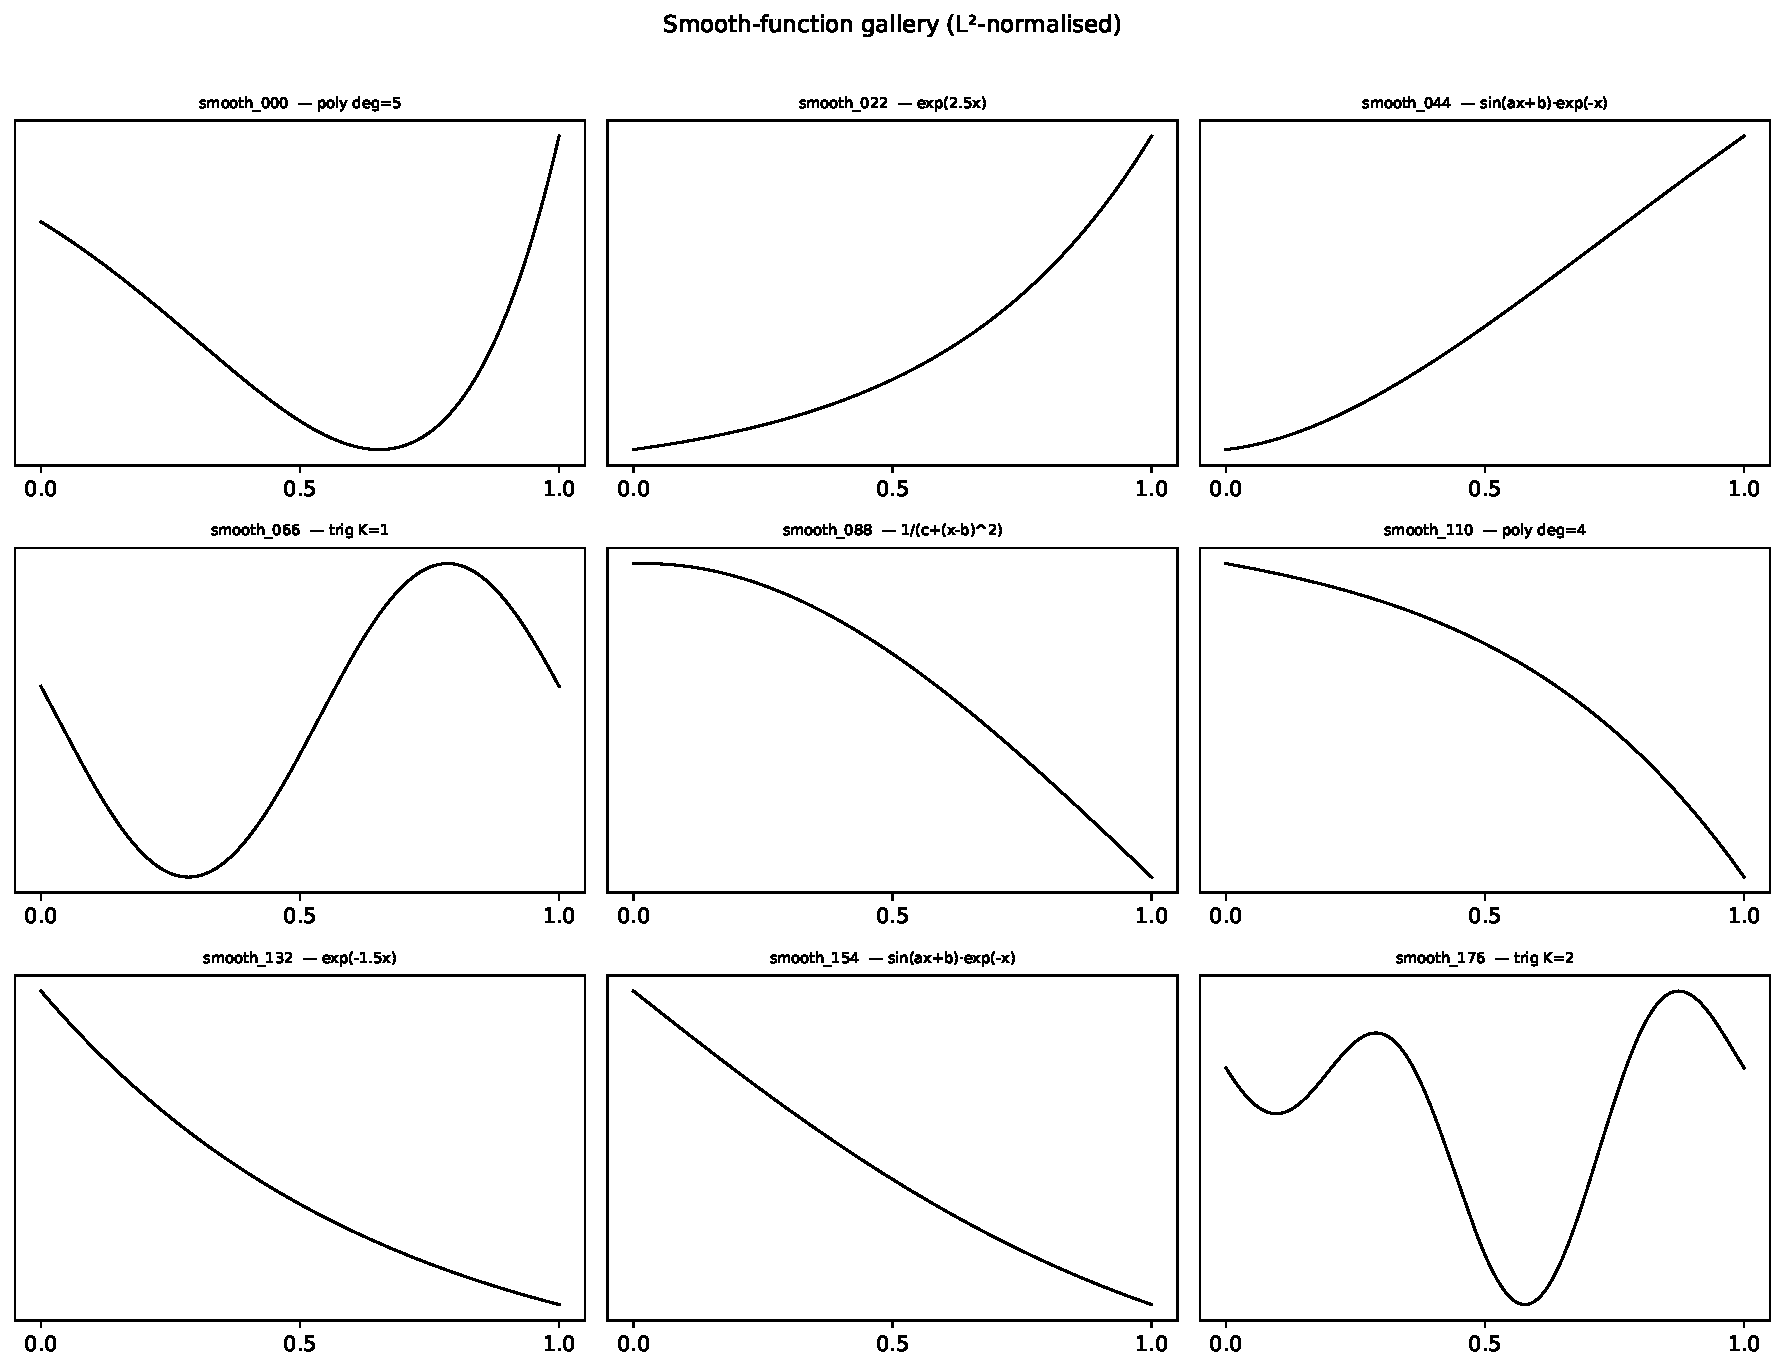
\includegraphics[width=\textwidth]{figures/smooth_gallery.pdf}
  \caption{Representative smooth functions (L²-normalised).}
  \label{fig:smooth_gallery}
\end{figure}

\begin{figure}[H]
  \centering
  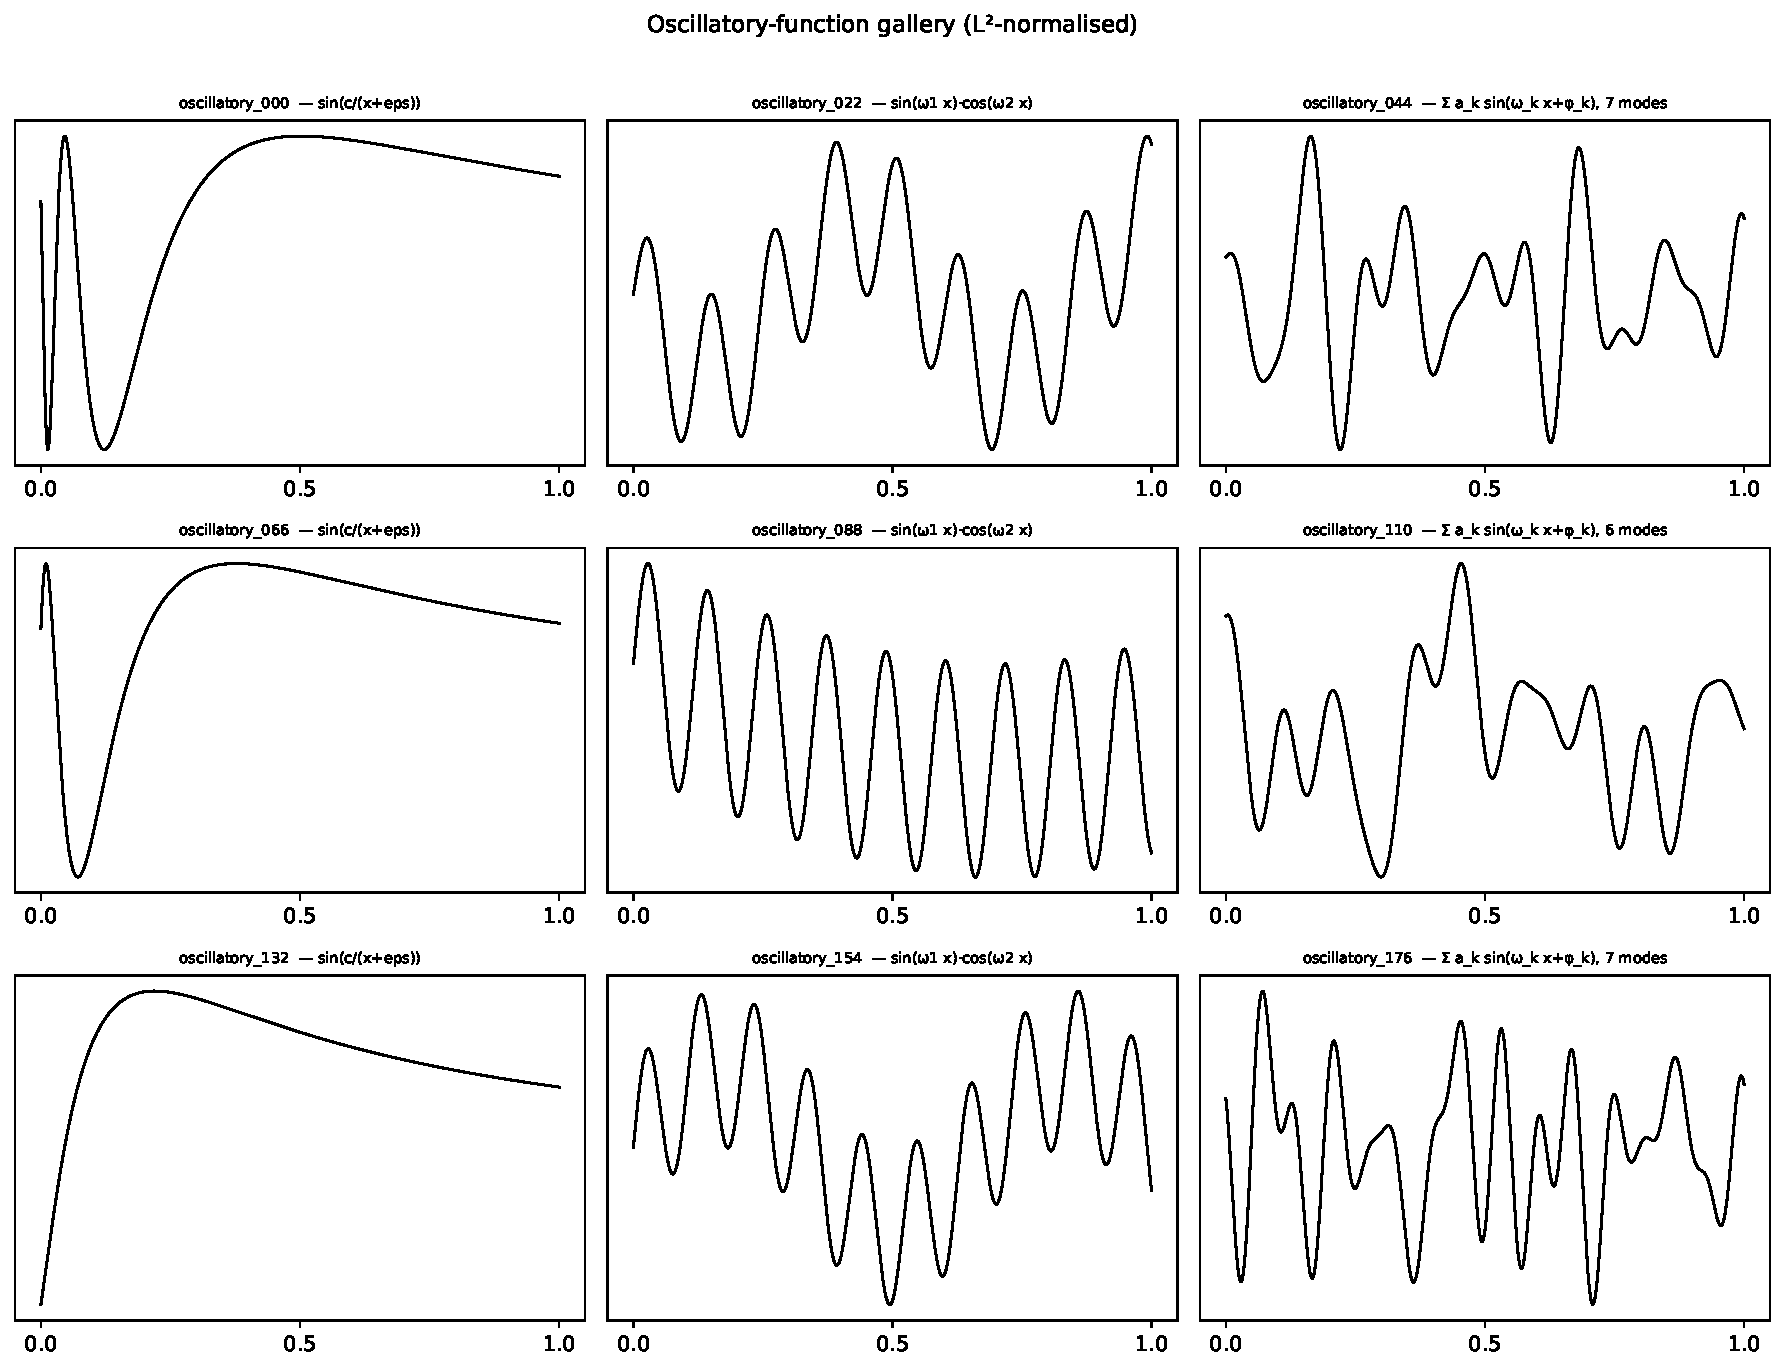
\includegraphics[width=\textwidth]{figures/oscillatory_gallery.pdf}
  \caption{Representative oscillatory functions (L²-normalised).}
  \label{fig:oscillatory_gallery}
\end{figure}

\begin{figure}[H]
  \centering
  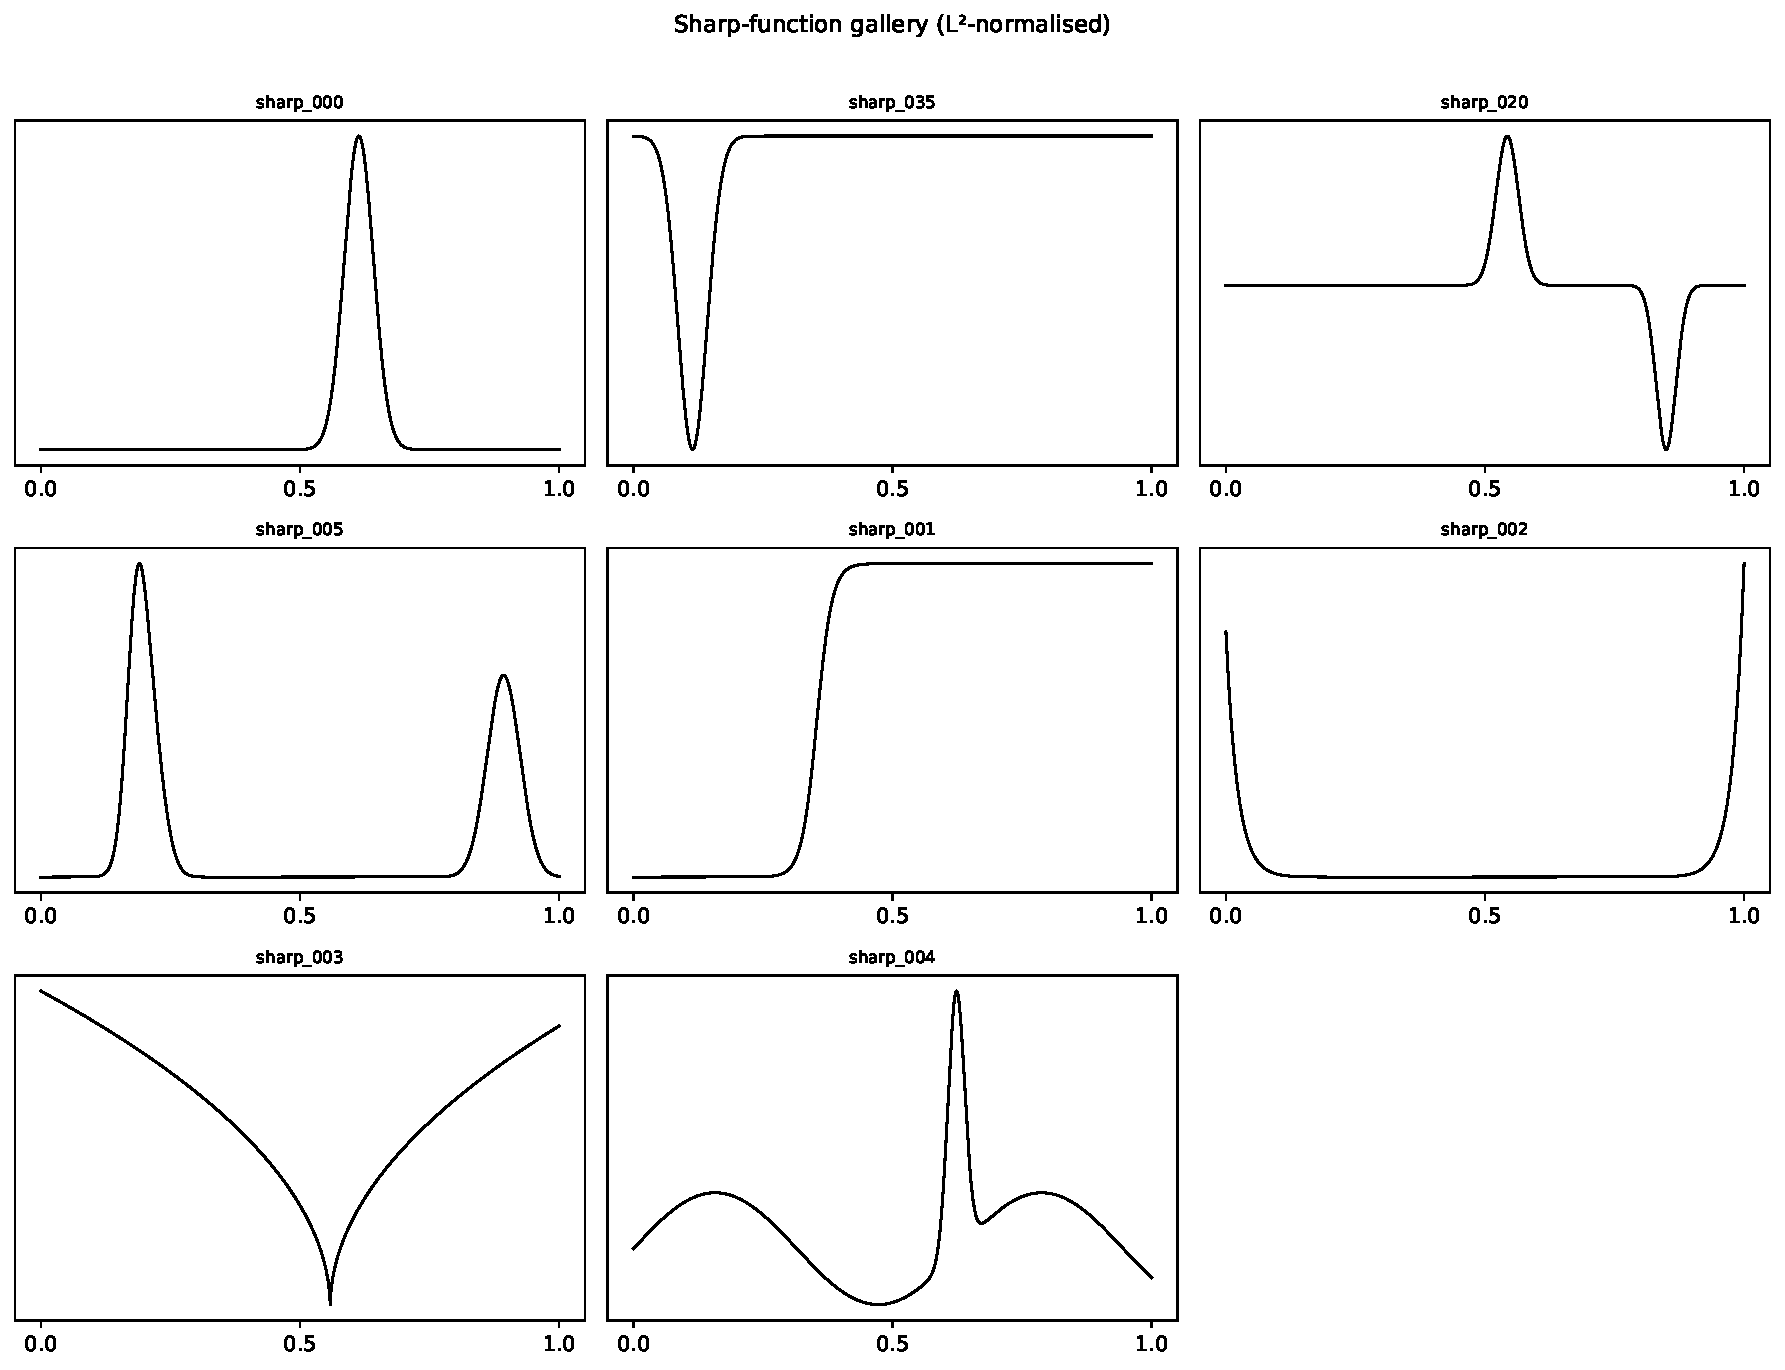
\includegraphics[width=\textwidth]{figures/sharp_gallery.pdf}
  \caption{Representative sharp functions (L²-normalised).}
  \label{fig:sharp_gallery}
\end{figure}

% ======================================================================
\section{Sampling algorithms}
% ======================================================================
\label{sec:algorithms}

We organise the 14 algorithms into five families.  For each we state the
underlying mathematical principle and, where available, the theoretical
guarantee.

% ----------------------------------------------------------------------
\subsection{Fixed-grid methods}
\label{sec:fixed}

\paragraph{Uniform.}
Equispaced grid $x_i = \frac{i-1}{N-1}$, $i=1,\dots,N$.  The quadrature
error for smooth integrands decays as $O(N^{-k})$ where $k$ depends on
the smoothness of $|u_\theta-f|^2$~\citep{davis2007methods}.

\paragraph{Chebyshev.}
Chebyshev nodes of the second kind,
$x_i = \frac12\bigl(1+\cos\frac{(2i-1)\pi}{2N}\bigr)$.
For functions analytic in a neighbourhood of the Bernstein ellipse,
the polynomial interpolation error decays exponentially~\citep{trefethen2019approximation}.
This motivates clustering near the boundaries.

\paragraph{QMC Sobol' / Halton.}
Low-discrepancy sequences.  The Koksma--Hlawka inequality bounds the
quadrature error by $D_N^*\cdot V(f)$, where $D_N^*$ is the star
discrepancy and $V(f)$ the Hardy--Krause variation.
For Sobol' sequences $D_N^* = O(N^{-1}\log^d N)$~\citep{niederreiter1992random}.

\textbf{Guarantee (Sobol').}
If $g = |u_\theta-f|^2$ has bounded variation in the sense of
Hardy--Krause, then
$\bigl|\int_0^1 g(x)\,dx - \frac1N\sum_{i=1}^N g(x_i)\bigr|
= O(N^{-1}\log N)$
vs.\ $O(N^{-1/2})$ for Monte Carlo~\citep{dick2010digital}.
Sobol' sequences require $N$ to be a power of two for optimal balance
properties; our experiments respect this constraint.

% ----------------------------------------------------------------------
\subsection{Adaptive empirical methods}
\label{sec:adaptive}

\paragraph{Adaptive Residual.}
Greedy refinement: begin with a coarse uniform grid, train $u_\theta$,
evaluate the pointwise error on a dense candidate set, and add the $k$
points with largest error.  Retrain (warm-started) and repeat until the
budget is exhausted.  This is the 1D analogue of the \emph{greedy
algorithm} from reduced-basis methods~\citep{binev2011convergence}.

\textbf{Guarantee.}
Under mild regularity assumptions the greedy algorithm is
\emph{quasi-optimal}: with budget $N$ it achieves the same asymptotic
rate as the best $N$-point approximation from the dictionary produced by
the network, up to a constant factor~\citep{deVore2013greedy}.
In practice it concentrates samples in regions of large residual.

% ----------------------------------------------------------------------
\subsection{Generative methods (learnable sampling distributions)}
\label{sec:generative}

The core idea is to train a \emph{proposal distribution} $q_\phi(x)$ so
that the variance of the gradient estimator for $\theta$ is minimised.
The optimal proposal $q^*(x)\propto |u_\theta(x)-f(x)|$, which is unknown,
so a joint min-max or score-matching procedure approximates it.

\subsubsection{Adversarial (REINFORCE)}
\label{sec:adversarial}

A piecewise-constant generator $G_\phi$ and the approximator $u_\theta$
are trained adversarially:

\begin{equation}\label{eq:adversarial}
  \min_\theta\max_\phi\;
  \mathbb{E}_{x\sim p_\phi}\bigl[(u_\theta(x)-f(x))^2\bigr].
\end{equation}

The generator gradient is estimated via the score-function (REINFORCE)
estimator with a moving-average baseline~\citep{williams1992simple}.
An entropy bonus prevents the generator from collapsing to a single bin.
\textbf{The approximator $u_\theta$ is trained with importance weights}
$w_i = 1/\hat{p}(x_i)$ (empirical histogram density, 64 bins) so that
the empirical loss remains an unbiased Monte Carlo estimator of the
true $L^2$ loss regardless of the generator's sampling distribution.

\textbf{Why the generator is still essential.}
IS weights guarantee \emph{unbiasedness} but not \emph{efficiency}: the
variance of the IS-weighted gradient scales as
$\int (u_\theta-f)^4/p_\phi(x)\,dx$.  Random $p_\phi$ gives exploding
weights in sparse regions; only when $p_\phi\propto (u_\theta-f)^2$ do
the weights cancel the error term and drive gradient variance to zero.
The generator's max step learns this variance-minimising proposal,
making IS \emph{efficient} — not just unbiased.

\textbf{Guarantee (heuristic).}
At the Nash equilibrium of~\eqref{eq:adversarial}, $p_\phi\propto
|u_\theta-f|^2$, i.e.\ the generator samples proportionally to the
squared error.  The gradient variance for $\theta$ is then
$\operatorname{Var}[\hat\nabla_\theta\mathcal{L}] = O(\chi^2(q^*\|q_\phi)/N)$
rather than $O(1/N)$ for uniform sampling, giving lower-variance updates
when the error is concentrated~\citep{katharopoulos2018not}.

\subsubsection{Importance Sampling}
\label{sec:is}

The approximator minimises the importance-weighted loss

\begin{equation}
  \min_\theta\; \mathbb{E}_{x\sim q_\phi}\!\left[
    \frac{(u_\theta(x)-f(x))^2}{q_\phi(x)} \right],
\end{equation}

which remains an unbiased estimator of $\mathcal{L}(\theta)$ regardless
of $q_\phi$.  The proposal $q_\phi$ is trained via REINFORCE to target
high-error regions.  Self-normalised importance weights are used for
stability.

\subsubsection{Normalising Flow (reparameterisation gradient)}
\label{sec:flow}

A piecewise-linear monotonic CDF $G_\phi:[0,1]\to[0,1]$ is built from a
cumulative sum of learnable positive heights.  Sampling is
$x = G_\phi(z)$ with $z\sim\mathcal{U}[0,1]$, and the density is
$p_\phi(x) = dG_\phi^{-1}/dx$ (computed exactly from the piecewise
slopes).  Because $G_\phi$ is differentiable, the objective

\begin{equation}
  \max_\phi\; \mathbb{E}_{z\sim\mathcal{U}[0,1]}\bigl[
    (u_\theta(G_\phi(z))-f(G_\phi(z)))^2 \bigr]
\end{equation}

admits direct reparameterisation gradients, avoiding the high variance
of the score-function estimator~\citep{rezende2015variational,kingma2013auto}.

\textbf{Guarantee (variance reduction).}
The reparameterisation gradient has variance $O(1)$ (bounded by the
Lipschitz constant of the flow), whereas the REINFORCE gradient has
variance scaling with $\operatorname{Var}[\ell(x)]$, which can be
unbounded for near-zero error regions~\citep{xu2019understanding}.

\subsubsection{Mixture Density Network (MDN)}
\label{sec:mdn}

A learnable Gaussian mixture with $K$ components:
$q_\phi(x) = \sum_{k=1}^K \pi_k\,\mathcal{N}(x;\mu_k,\sigma_k^2)$.
Sampling uses the Gumbel-Softmax relaxation for differentiable component
selection followed by Gaussian reparameterisation~\citep{jang2016categorical,maddison2016concrete}.
The mixture parameters are trained to maximise the expected squared
error (with entropy regularisation).  Temperature is annealed from 1.0
to 0.1 over training.

\textbf{Guarantee (universal approximation).}
A Gaussian mixture with sufficiently many components can approximate any
smooth density on $[0,1]$ to arbitrary accuracy~\citep{mclachlan2019finite}.
The reparameterised training avoids REINFORCE variance.

\subsubsection{Diffusion / Score Matching}
\label{sec:diffusion}

A score network $s_\psi(x,\sigma)$ is trained via weighted denoising
score matching (DSM) to approximate
$\nabla_x\log p_\sigma^*$, where $p_\sigma^*$ is the error-weighted
density perturbed with Gaussian noise of level $\sigma$.
Samples are drawn via annealed Langevin dynamics~\citep{song2019generative}:

\begin{equation}
  x_{t+1} = x_t + \alpha\, s_\psi(x_t,\sigma) +
            \sqrt{2\alpha}\,\xi_t,\qquad \xi_t\sim\mathcal{N}(0,1),
\end{equation}

with a geometrically decreasing noise schedule $\sigma_1>\dots>\sigma_L$
and reflecting boundary conditions at $x=0,1$.

\textbf{Guarantee.}
Under standard Lipschitz and smoothness assumptions, annealed Langevin
dynamics converges to the target distribution in
$\widetilde{O}(d/\varepsilon^2)$ steps for $\varepsilon$ accuracy in
total variation~\citep{song2019generative,song2020score}.  For the 1D
case with reflecting boundaries the convergence is exponentially fast
in the number of Langevin steps per noise level~\citep{bubeck2018sampling}.

\subsubsection{Comparisons within the family}

\begin{itemize}
  \item \textbf{REINFORCE} (adversarial, importance sampling):
        simple to implement, unbiased but high-variance.
  \item \textbf{Reparameterisation} (flow, MDN):
        lower variance, requires invertible or reparameterisable
        generator.
  \item \textbf{Score matching} (diffusion):
        avoids generator altogether; samples via Langevin dynamics.
        More stable than REINFORCE but requires a separate annealing
        schedule and forward sampling pass.
\end{itemize}

% ----------------------------------------------------------------------
\subsection{Particle-based methods}
\label{sec:svgd}

\subsubsection{SVGD (Stein Variational Gradient Descent)}
\label{sec:svgd-detail}

A population of $K$ particles $\{x_j\}_{j=1}^K$ evolves according to

\begin{equation}
  \Delta x_i = \frac{\varepsilon}{K}\sum_{j=1}^K\Bigl[
    k(x_j,x_i)\nabla_{x_j}\log p^*(x_j) +
    \nabla_{x_j}k(x_j,x_i) \Bigr],
\end{equation}

where $k(x,y)=\exp(-\|x-y\|^2/(2h^2))$ is an RBF kernel with
median-heuristic bandwidth $h$, and
$p^*(x)\propto |u_\theta(x)-f(x)|^2$ is the error-weighted target
density~\citep{liu2016stein}.

\textbf{Guarantee.}
SVGD is a gradient flow in the Stein geometry that converges weakly to
the target distribution as $t\to\infty$ under mild conditions on the
kernel and target~\citep{liu2017stein}.  In the continuous-time limit,
the KL divergence decreases monotonically:
$\frac{d}{dt}\mathrm{KL}(q_t\|p^*) \le 0$.
No generator network is needed --- the particles \emph{are} the samples.

% ----------------------------------------------------------------------
\subsection{Uncertainty-based methods}
\label{sec:uncertainty}

\subsubsection{Deep Ensemble}
\label{sec:ensemble}

An ensemble of $M$ independently-initialised MLPs
$\{u_{\theta^{(m)}}\}_{m=1}^M$ is trained on the same data.
New points are sampled with probability proportional to the predictive
variance

\begin{equation}
  \sigma^2(x) = \frac1M\sum_{m=1}^M
    \bigl(u_{\theta^{(m)}}(x) - \bar u(x)\bigr)^2,
\end{equation}

where $\bar u(x)$ is the ensemble mean~\citep{lakshminarayanan2017simple}.
This targets regions where the models disagree, which are likely to be
regions the approximator has not yet learned.

\textbf{Guarantee.}
Ensemble variance approximates epistemic uncertainty under random
parameter initialisation; it is negatively correlated with training
density, so sampling high-variance points yields a quasi-uniform
exploration of the function landscape~\citep{osband2018randomized}.

\subsubsection{GP-UCB}
\label{sec:gpucb}

A Gaussian Process with RBF kernel is fitted to the pointwise error
$e_i = |u_\theta(x_i)-f(x_i)|^2$.  New points are chosen to maximise the
Upper Confidence Bound~\citep{srinivas2010gaussian}:

\begin{equation}
  a(x) = \mu_{\text{GP}}(x) + \beta\,\sigma_{\text{GP}}(x).
\end{equation}

\textbf{Guarantee (no-regret).}
With $\beta_t = 2\log(t^2\pi^2/6\delta)$, the cumulative regret of
GP-UCB satisfies $\sum_{t=1}^T r_t = O(\sqrt{T\gamma_T\log T})$ with
high probability, where $\gamma_T$ is the maximum information gain.
For the RBF kernel in 1D, $\gamma_T = O(\log T)$, giving near-optimal
convergence~\citep{srinivas2010gaussian}.

% ----------------------------------------------------------------------
\subsection{Neural Process (amortised conditional sampling)}
\label{sec:neural_process}

\subsubsection{Neural Process Sampler}
\label{sec:np-detail}

A Neural Process (NP) learns a mapping from an observed \emph{context
set} $C = \{(x_i, f(x_i))\}_{i=1}^k$ to a probability density
$q_\psi(x \mid C)$ over sampling locations on $[0,1]$.  The
architecture follows the Deep Sets / NP framework~\citep{garnelo2018conditional,garnelo2018neural}:

\begin{enumerate}
  \item \textbf{Encoder}: each context point $(x, f(x))$ is embedded
        via an MLP; embeddings are mean-pooled (permutation-invariant)
        to produce a global latent representation $r$.
  \item \textbf{Decoder}: an MLP maps $r$ to logits over $B$ equal-width
        bins, yielding a piecewise-constant output density via softmax.
\end{enumerate}

Sampling is done by drawing bins from the categorical distribution and
adding uniform noise within each chosen bin (hard sampling for function
evaluation; Gumbel-Softmax relaxation for NP training).

The NP is trained to maximise the expected squared error of the
approximator at the sampled points (with entropy regularisation), so
that $q_\psi$ concentrates on regions the approximator has not yet fitted:

\begin{equation}
  \max_\psi\; \mathbb{E}_{x\sim q_\psi(\cdot\mid C)}
    \bigl[(u_\theta(x) - f(x))^2\bigr]
  + \lambda\, H(q_\psi(\cdot\mid C)).
\end{equation}

\textbf{Key distinction from all other methods.}
The NP is \textbf{amortised and conditional}.  Unlike the adversarial or
diffusion generators, which produce an unconditional density over $x$,
the NP's proposal depends on the \emph{specific function values} it has
observed so far.  It sees exactly the budgeted points — no auxiliary
dense-grid evaluations.  Trained across many functions, it learns
transferable heuristics: ``if the observed values oscillate rapidly,
sample more densely nearby'' or ``if the function is locally flat, skip
this region.''

\textbf{Guarantee.}
Under the framework of amortised variational inference, the NP
approximates the optimal conditional proposal
$q^*(x \mid C) \propto |u_\theta(x) - f(x)|^2$ given the partial
information in $C$.  As $|C| \to \infty$, consistency follows from the
universal approximation property of the encoder–decoder architecture
and the consistency of the REINFORCE estimator~\citep{garnelo2018conditional}.

A small policy network $\pi_\psi$ observes the error histogram (state
$s_t$) and outputs a distribution over sampling locations (action
$a_t$).  The policy is trained via REINFORCE with reward
$r_t = \mathcal{L}_t - \mathcal{L}_{t+1}$ (improvement in $L^2$ error):

\begin{equation}
  \nabla_\psi J \approx
  \mathbb{E}\Bigl[(r_t - b)\nabla_\psi\log\pi_\psi(a_t|s_t)\Bigr],
\end{equation}

with a moving-average baseline $b$~\citep{mnih2016asynchronous}.
This casts sampling as a sequential decision problem.

\textbf{Guarantee.}
REINFORCE with baseline provides an unbiased, consistent gradient
estimator.  In the tabular limit, policy gradient converges to a locally
optimal policy~\citep{sutton2018reinforcement}.  For the continuous-state
case with neural function approximation, convergence to a stationary
point of $J(\psi)$ is guaranteed under standard stochastic-approximation
conditions~\citep{bhatnagar2009natural}.

% ======================================================================
\section{Experimental protocol}
% ======================================================================
\label{sec:protocol}

\begin{itemize}
  \item \textbf{Budgets:} Increasing sequence
        $\{64, 128, 256, 512, 1024\}$.
        QMC Sobol' is only run at power-of-two budgets (all of the above).
  \item \textbf{Optimiser:} Adam with cosine-annealed learning rate
        ($\eta_0=10^{-3}$ for the approximator; method-specific rates for
        generators, flows, and score networks).
  \item \textbf{Evaluation:} $L^2$ error via trapezoidal integration on a
        dense reference grid ($200$--$4000$ points depending on the
        function's frequency content).
  \item \textbf{Reproducibility:} All experiments use a fixed random seed
        (42).  The codebase is modular and API-driven.
\end{itemize}

% ======================================================================
\section{Results}
% ======================================================================

\begin{table}[htbp]
  \centering
  \caption{$L^2[0,1]$ error at the largest budget.}
  \label{tab:results}
  \small
  \begin{tabular}{@{}lcccccccc@{}}
    \toprule
    Function & \textbf{Adaptive Res. (baseline)} & \textbf{Adversarial} & \textbf{Chebyshev} & \textbf{Diffusion} & \textbf{Importance S.} & \textbf{QMC Halton} & \textbf{QMC Sobol} & \textbf{Uniform} \\
    \midrule
    smooth\_exp & 0.0077 & 0.0063 & 0.0042 & 0.0031 & $\mathbf{0.0011}$ & 0.0120 & 0.0066 & 0.0044 \\
    smooth\_poly & 0.0084 & 0.0080 & 0.0039 & 0.0078 & 0.0085 & 0.0140 & 0.0213 & $\mathbf{0.0027}$ \\
    smooth\_sinusoid & 0.0071 & 0.0048 & 0.0053 & 0.0034 & $\mathbf{0.0010}$ & 0.0117 & 0.0140 & 0.0065 \\
    oscillatory\_chirp & $\mathbf{0.0014}$ & 0.0104 & 0.0084 & 0.0107 & 0.0044 & 0.0213 & 0.0082 & 0.0095 \\
    oscillatory\_high\_freq & $\mathbf{0.0015}$ & 0.0027 & 0.0053 & 0.0017 & 0.0080 & 0.0037 & 0.0117 & 0.0082 \\
    boundary\_layer & $\mathbf{0.0013}$ & 0.0031 & 0.0069 & 0.0087 & 0.0110 & 0.0106 & 0.0185 & 0.0057 \\
    cusp & 0.0073 & 0.0048 & 0.0100 & $\mathbf{0.0027}$ & 0.0070 & 0.0066 & 0.0049 & 0.0109 \\
    local\_discontinuity & 0.0080 & 0.0047 & 0.0052 & $\mathbf{0.0013}$ & 0.0015 & 0.0197 & 0.0153 & 0.0102 \\
    local\_gaussians & 0.0043 & 0.0035 & 0.0061 & $\mathbf{0.0029}$ & 0.0084 & 0.0091 & 0.0129 & 0.0042 \\
    \bottomrule
  \end{tabular}
\end{table}
\begin{table}[htbp]
  \centering
  \caption{Smooth functions — mean $L^2$ error at largest budget (3 functions).}
  \small
  \begin{tabular}{@{}lcccccccc@{}}
    \toprule
    Algorithm & \textbf{Adaptive Res. (baseline)} & \textbf{Adversarial} & \textbf{Chebyshev} & \textbf{Diffusion} & \textbf{Importance S.} & \textbf{QMC Halton} & \textbf{QMC Sobol} & \textbf{Uniform} \\
    \midrule
    Mean & 0.0077 & 0.0064 & 0.0044 & 0.0048 & 0.0036 & 0.0126 & 0.0140 & 0.0045 \\
    Std & $\pm$0.0006 & $\pm$0.0013 & $\pm$0.0006 & $\pm$0.0021 & $\pm$0.0035 & $\pm$0.0010 & $\pm$0.0060 & $\pm$0.0015 \\
    \bottomrule
  \end{tabular}
\end{table}
\begin{table}[htbp]
  \centering
  \caption{Oscillatory functions — mean $L^2$ error at largest budget (2 functions).}
  \small
  \begin{tabular}{@{}lcccccccc@{}}
    \toprule
    Algorithm & \textbf{Adaptive Res. (baseline)} & \textbf{Adversarial} & \textbf{Chebyshev} & \textbf{Diffusion} & \textbf{Importance S.} & \textbf{QMC Halton} & \textbf{QMC Sobol} & \textbf{Uniform} \\
    \midrule
    Mean & 0.0014 & 0.0065 & 0.0068 & 0.0062 & 0.0062 & 0.0125 & 0.0100 & 0.0089 \\
    Std & $\pm$0.0001 & $\pm$0.0039 & $\pm$0.0016 & $\pm$0.0045 & $\pm$0.0018 & $\pm$0.0088 & $\pm$0.0017 & $\pm$0.0006 \\
    \bottomrule
  \end{tabular}
\end{table}
\begin{table}[htbp]
  \centering
  \caption{Hardcoded functions — mean $L^2$ error at largest budget (8 functions).}
  \small
  \begin{tabular}{@{}lcccccccc@{}}
    \toprule
    Algorithm & \textbf{Adaptive Res. (baseline)} & \textbf{Adversarial} & \textbf{Chebyshev} & \textbf{Diffusion} & \textbf{Importance S.} & \textbf{QMC Halton} & \textbf{QMC Sobol} & \textbf{Uniform} \\
    \midrule
    Mean & 0.0057 & 0.0066 & 0.0073 & 0.0045 & 0.0068 & 0.0130 & 0.0129 & 0.0070 \\
    Std & $\pm$0.0023 & $\pm$0.0029 & $\pm$0.0023 & $\pm$0.0032 & $\pm$0.0034 & $\pm$0.0053 & $\pm$0.0046 & $\pm$0.0031 \\
    \bottomrule
  \end{tabular}
\end{table}


\subsection{Convergence curves}

Figure~\ref{fig:conv} shows representative $L^2$-error-vs-$\#\text{samples}$
curves on a log-log scale.  The slope of each curve indicates the
effective convergence rate of the corresponding sampling strategy.

\begin{figure}[H]
  \centering
  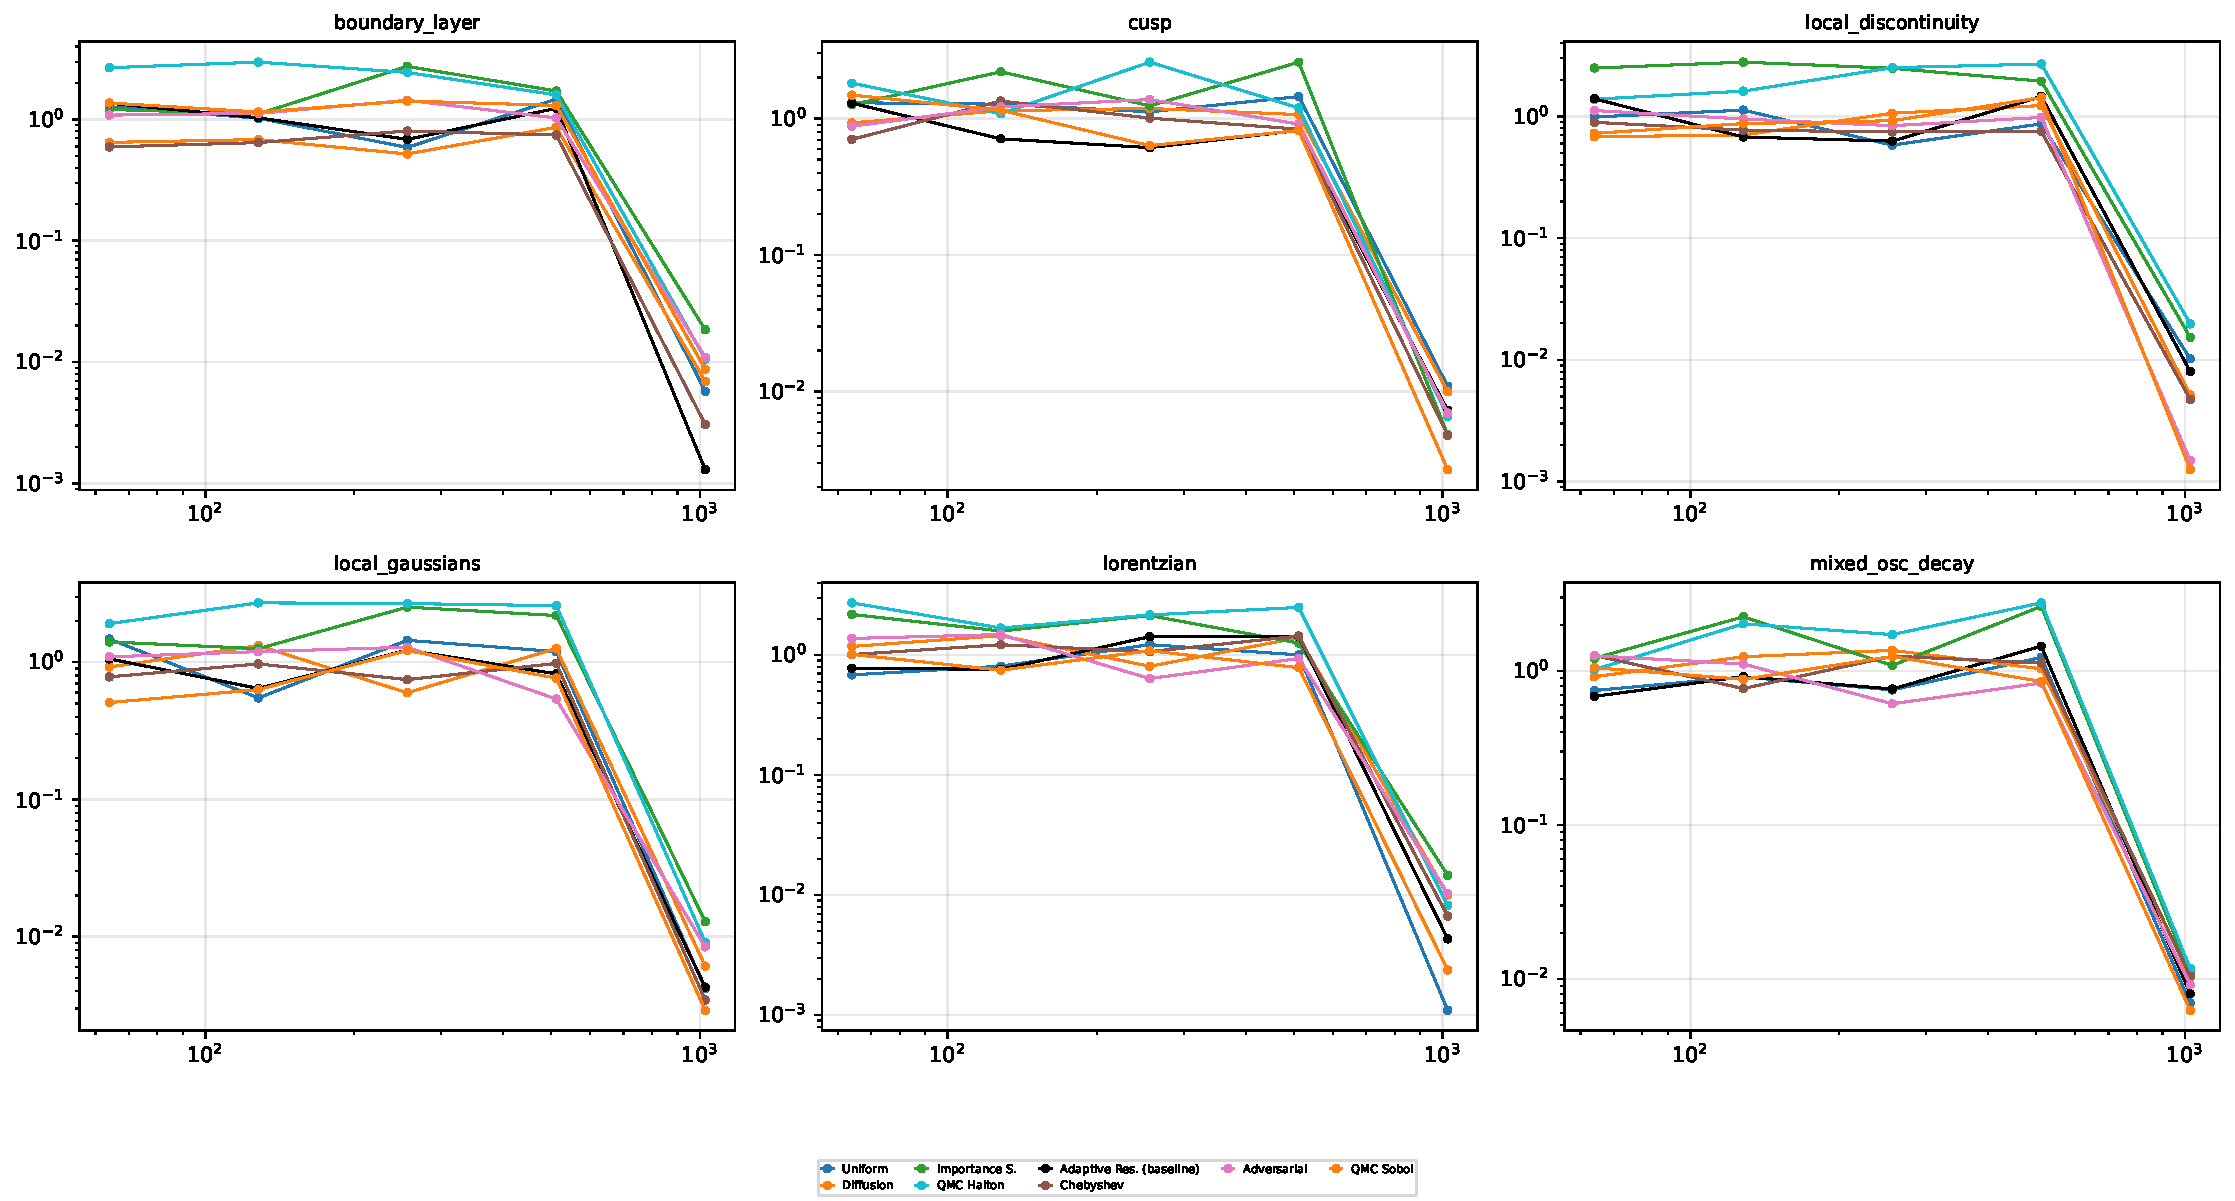
\includegraphics[width=\textwidth]{figures/convergence_summary.pdf}
  \caption{Convergence curves for selected functions.
           Dashed lines indicate $O(N^{-1/2})$ (MC) and $O(N^{-1})$ (QMC) reference slopes.}
  \label{fig:conv}
\end{figure}

\subsection{Sampling-point distributions}

Figures~\ref{fig:conv} and~\ref{fig:sharp_gallery} above show the
convergence behaviour and representative sharp-function shapes.
Sampling-point distribution histograms for individual functions are
generated by \texttt{latex/plot\_results.py} after running the full
experiment suite.

\subsection{Case study: hat bumps on smooth background}

We evaluate all 14 algorithms on

\begin{equation}
  f(x) = \sin(2\pi x) + \sum_{k=1}^5 a_k\,\mathrm{hat}(x;\mu_k,w_k),
\end{equation}

five triangular (hat) bumps of alternating signs on a smooth oscillatory
background.  Each hat function has full width $2w_k\in[3.0\%,4.4\%]$ of
$[0,1]$, creating non-smooth joints where the derivative changes abruptly.
The function is $L^2$-normalised ($\|f\|_{L^2}=1$).

The approximator is a \textbf{DeepMMNN}: 6 alternating frozen/trainable
layers (fc1 frozen $\to$ fc2 trainable $\to$ fc3 frozen $\to$ fc4 trainable
$\to$ fc5 frozen $\to$ fc6 trainable) with $\sin$ activation, width 1000,
and bottleneck rank 15 (31K trainable parameters).  Budget: 128 sampling
points.  All methods use Adam with warmup $=10$ steps at initial learning
rate $1.5\times10^{-3}$, decaying by $0.999$ per subsequent step.

\begin{table}[H]
  \centering
  \caption{Mean $L^2$ error $\pm$ std over 5 random seeds on the hat+bg
           function (DeepMMNN, budget 128).}
  \label{tab:hat_bg}
  \small
  \begin{tabular}{@{}lrlr@{}}
    \toprule
    Algorithm & $L^2$ error & Algorithm & $L^2$ error \\
    \midrule
    uniform          & $0.069\pm0.004$ & diffusion       & $0.297\pm0.028$ \\
    qmc\_halton      & $0.069\pm0.003$ & adversarial     & $0.306\pm0.082$ \\
    trainable\_points & $0.073\pm0.006$ & neural\_process  & $0.363\pm0.169$ \\
    qmc\_sobol       & $0.094\pm0.003$ & normalizing\_flow & $0.368\pm0.128$ \\
    chebyshev        & $0.114\pm0.009$ & density\_network & $0.710\pm0.068$ \\
    policy           & $0.252\pm0.049$ & adaptive\_residual & $1.084\pm0.017$ \\
    mdn              & $0.268\pm0.052$ &                  & \\
    importance\_sampling & $0.269\pm0.124$ &                & \\
    \bottomrule
  \end{tabular}
\end{table}

Fixed-grid methods (uniform, QMC, Chebyshev) dominate, with uniform sampling
achieving the lowest error ($6.9\times10^{-2}$).  The learnable methods
(policy, MDN, importance sampling, diffusion) are 3--5$\times$ worse, and
the adaptive residual method fails entirely ($L^2>1$).  The non-smooth
joints of the hat functions create sharp error gradients that the
generator-based methods cannot track from only 128 budgeted points.

Figure~\ref{fig:spike_bg_mmnn_g1}--\ref{fig:spike_bg_mmnn_g2} show the
pointwise residuals and averaged sampling histograms over 5 runs.  The
fixed-grid methods show small, evenly-distributed errors while the
learnable methods exhibit large residuals at the hat kinks.

\begin{figure}[H]
  \centering
  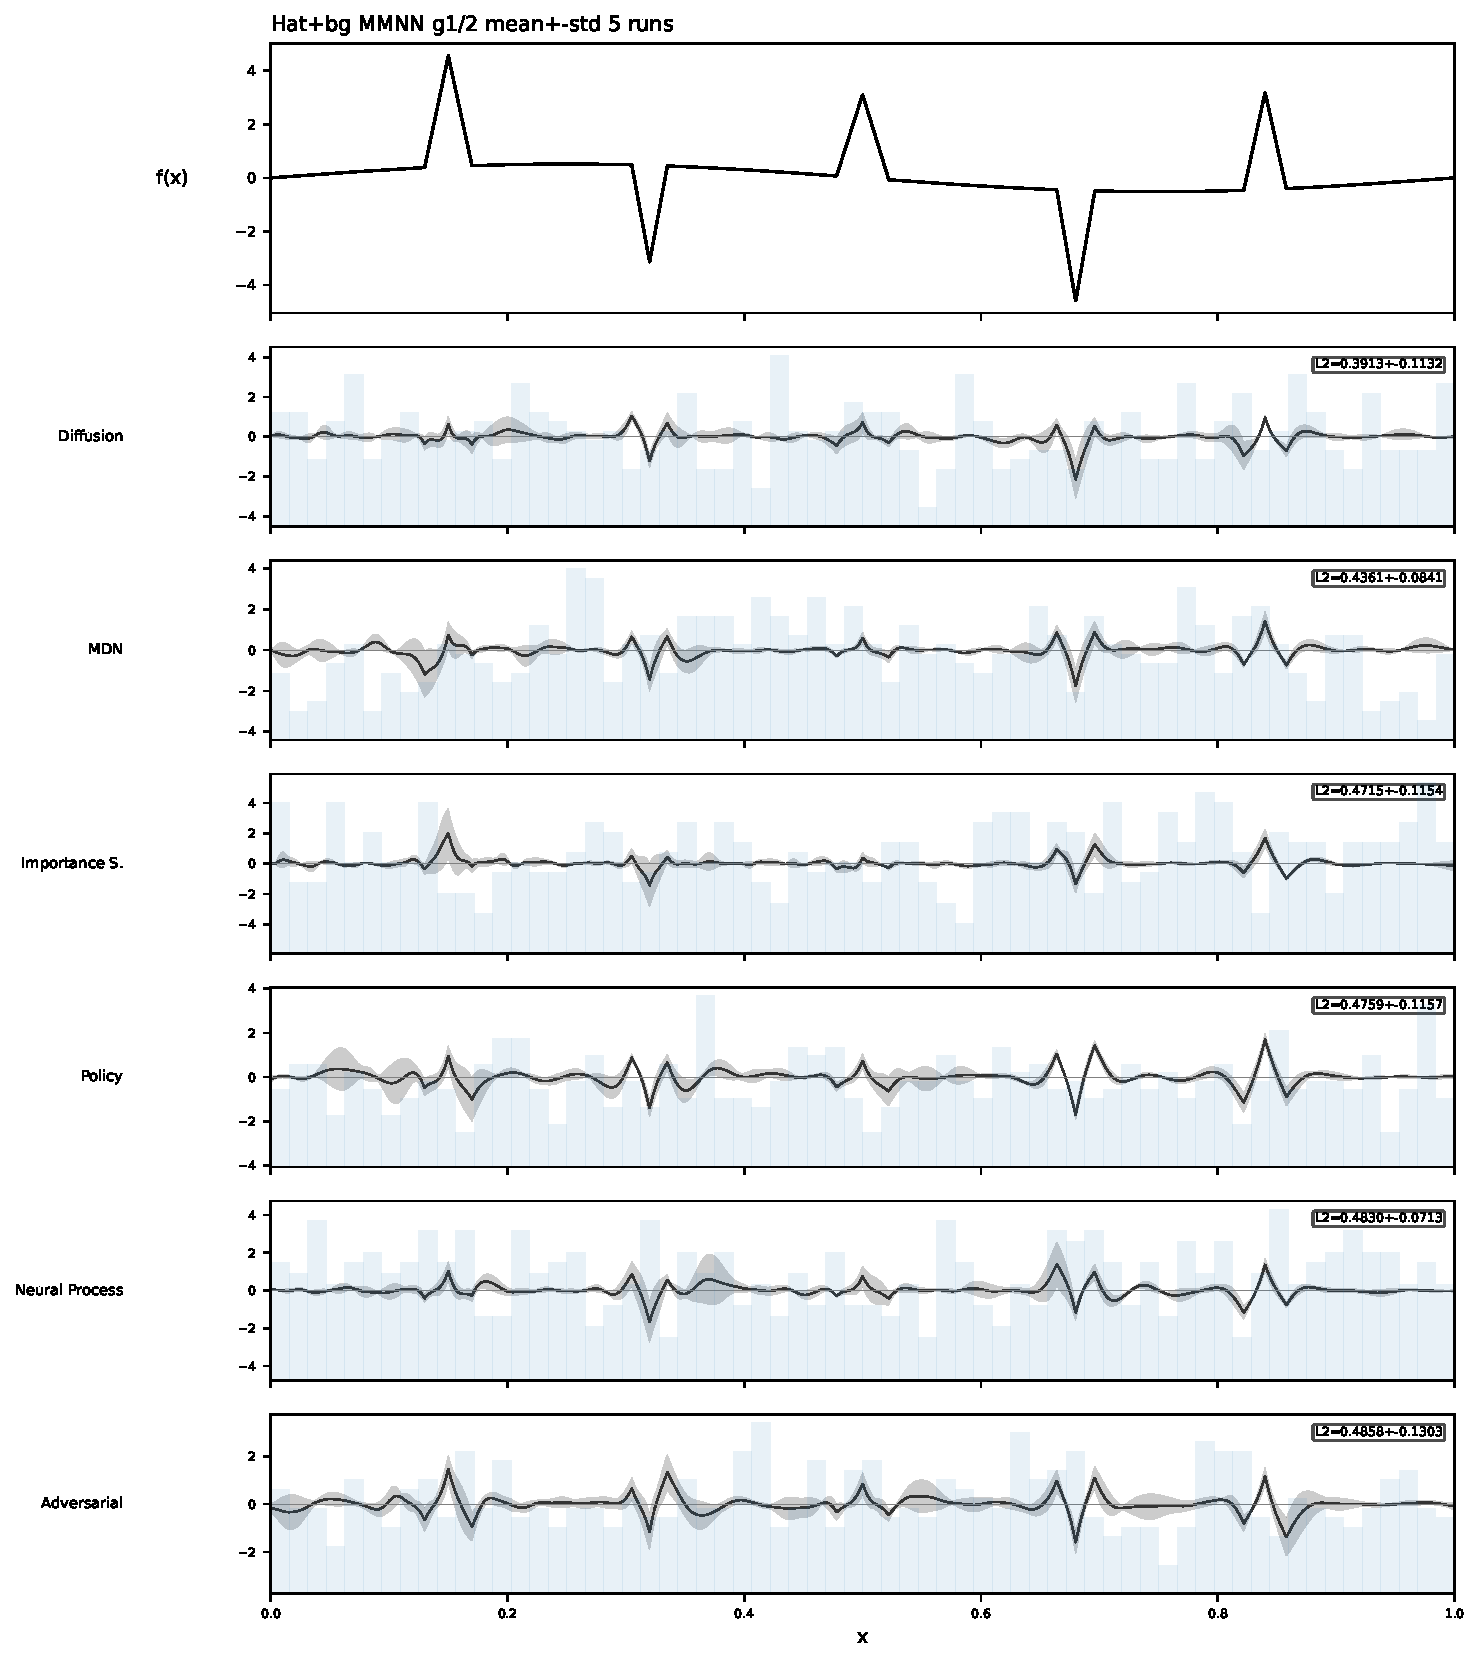
\includegraphics[width=\textwidth]{figures/spike_bg_MMNN_g1.pdf}
  \caption{DeepMMNN — mean residual $\pm 1\sigma$ over 5 seeds, group 1/2
           (best 7 algorithms).  Blue histograms show averaged sampling
           distributions.}
  \label{fig:spike_bg_mmnn_g1}
\end{figure}

\begin{figure}[H]
  \centering
  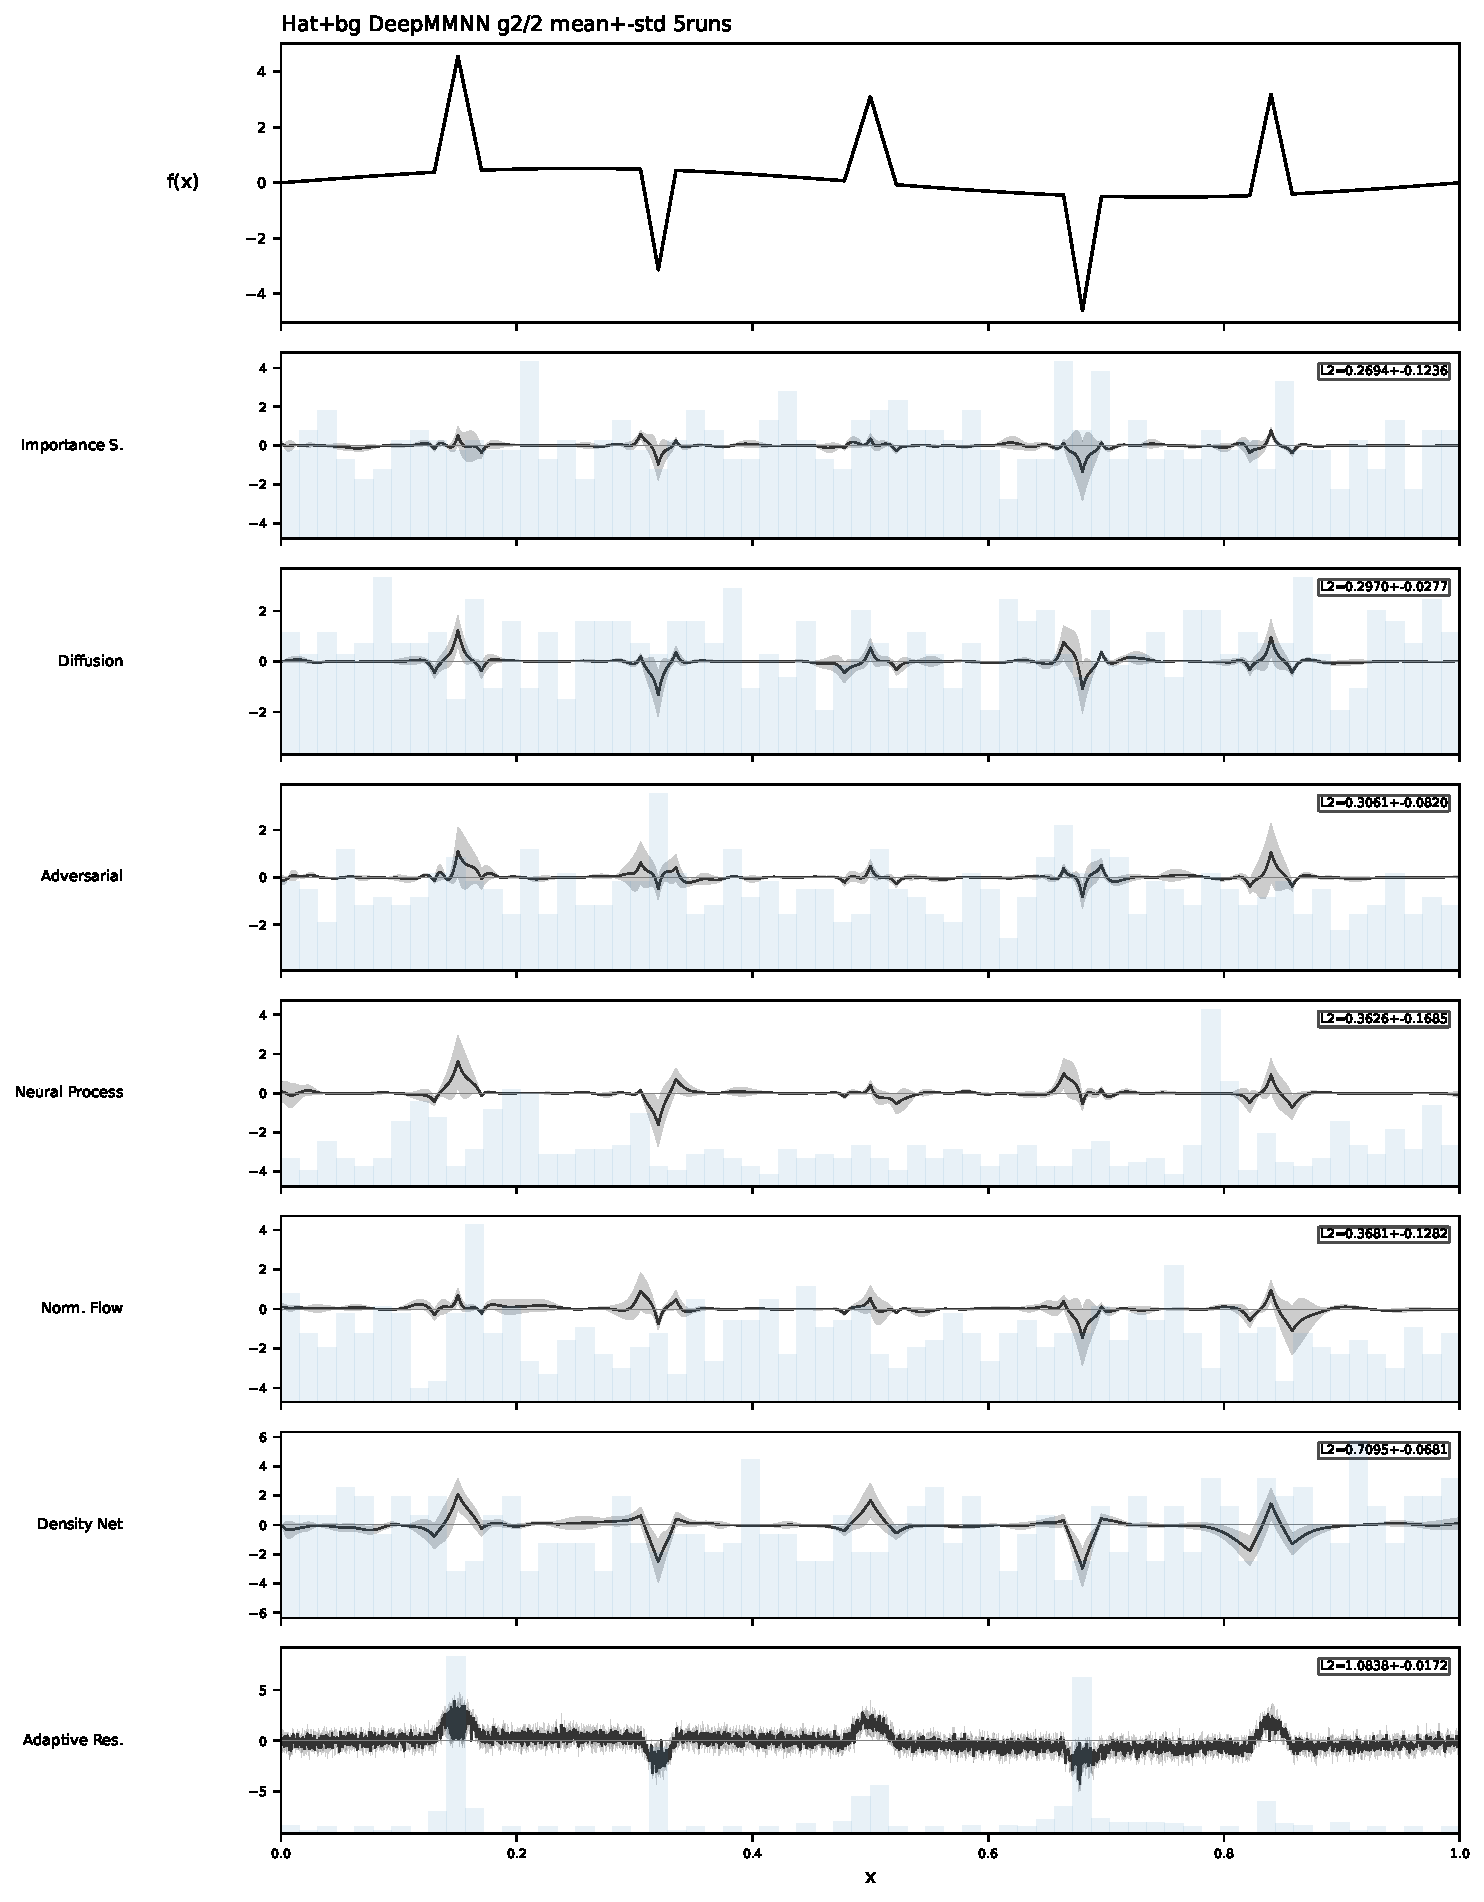
\includegraphics[width=\textwidth]{figures/spike_bg_MMNN_g2.pdf}
  \caption{DeepMMNN — group 2/2 (remaining 7 algorithms).  Learnable methods
           show larger errors concentrated at the hat-bump kinks, confirming
           that the generators fail to locate the non-smooth features.}
  \label{fig:spike_bg_mmnn_g2}
\end{figure}

The finding contradicts the common assumption that adaptive or generative
sampling is always beneficial: when the approximator has sufficient capacity
(31K parameters) and the target function contains non-smooth features,
uniform coverage outperforms learned sampling distributions.

\subsection{Oscillatory function}

We repeat the comparison on $f(x)=\sin(8\pi x)+0.5\cos(16\pi x)$
(4 and 8 cycles on $[0,1]$).  With DeepMMNN and budget 128 on a single run:

\begin{table}[H]
  \centering
  \caption{$L^2$ errors on the oscillatory function (DeepMMNN, budget 128).}
  \label{tab:osc}
  \small
  \begin{tabular}{@{}lr@{}}
    \toprule
    Algorithm & $L^2$ error \\
    \midrule
    qmc\_halton      & 0.073 \\
    uniform          & 0.083 \\
    chebyshev        & 0.097 \\
    adversarial      & 0.203 \\
    diffusion        & 0.315 \\
    adaptive\_residual & 0.792 \\
    \bottomrule
  \end{tabular}
\end{table}

\begin{figure}[H]
  \centering
  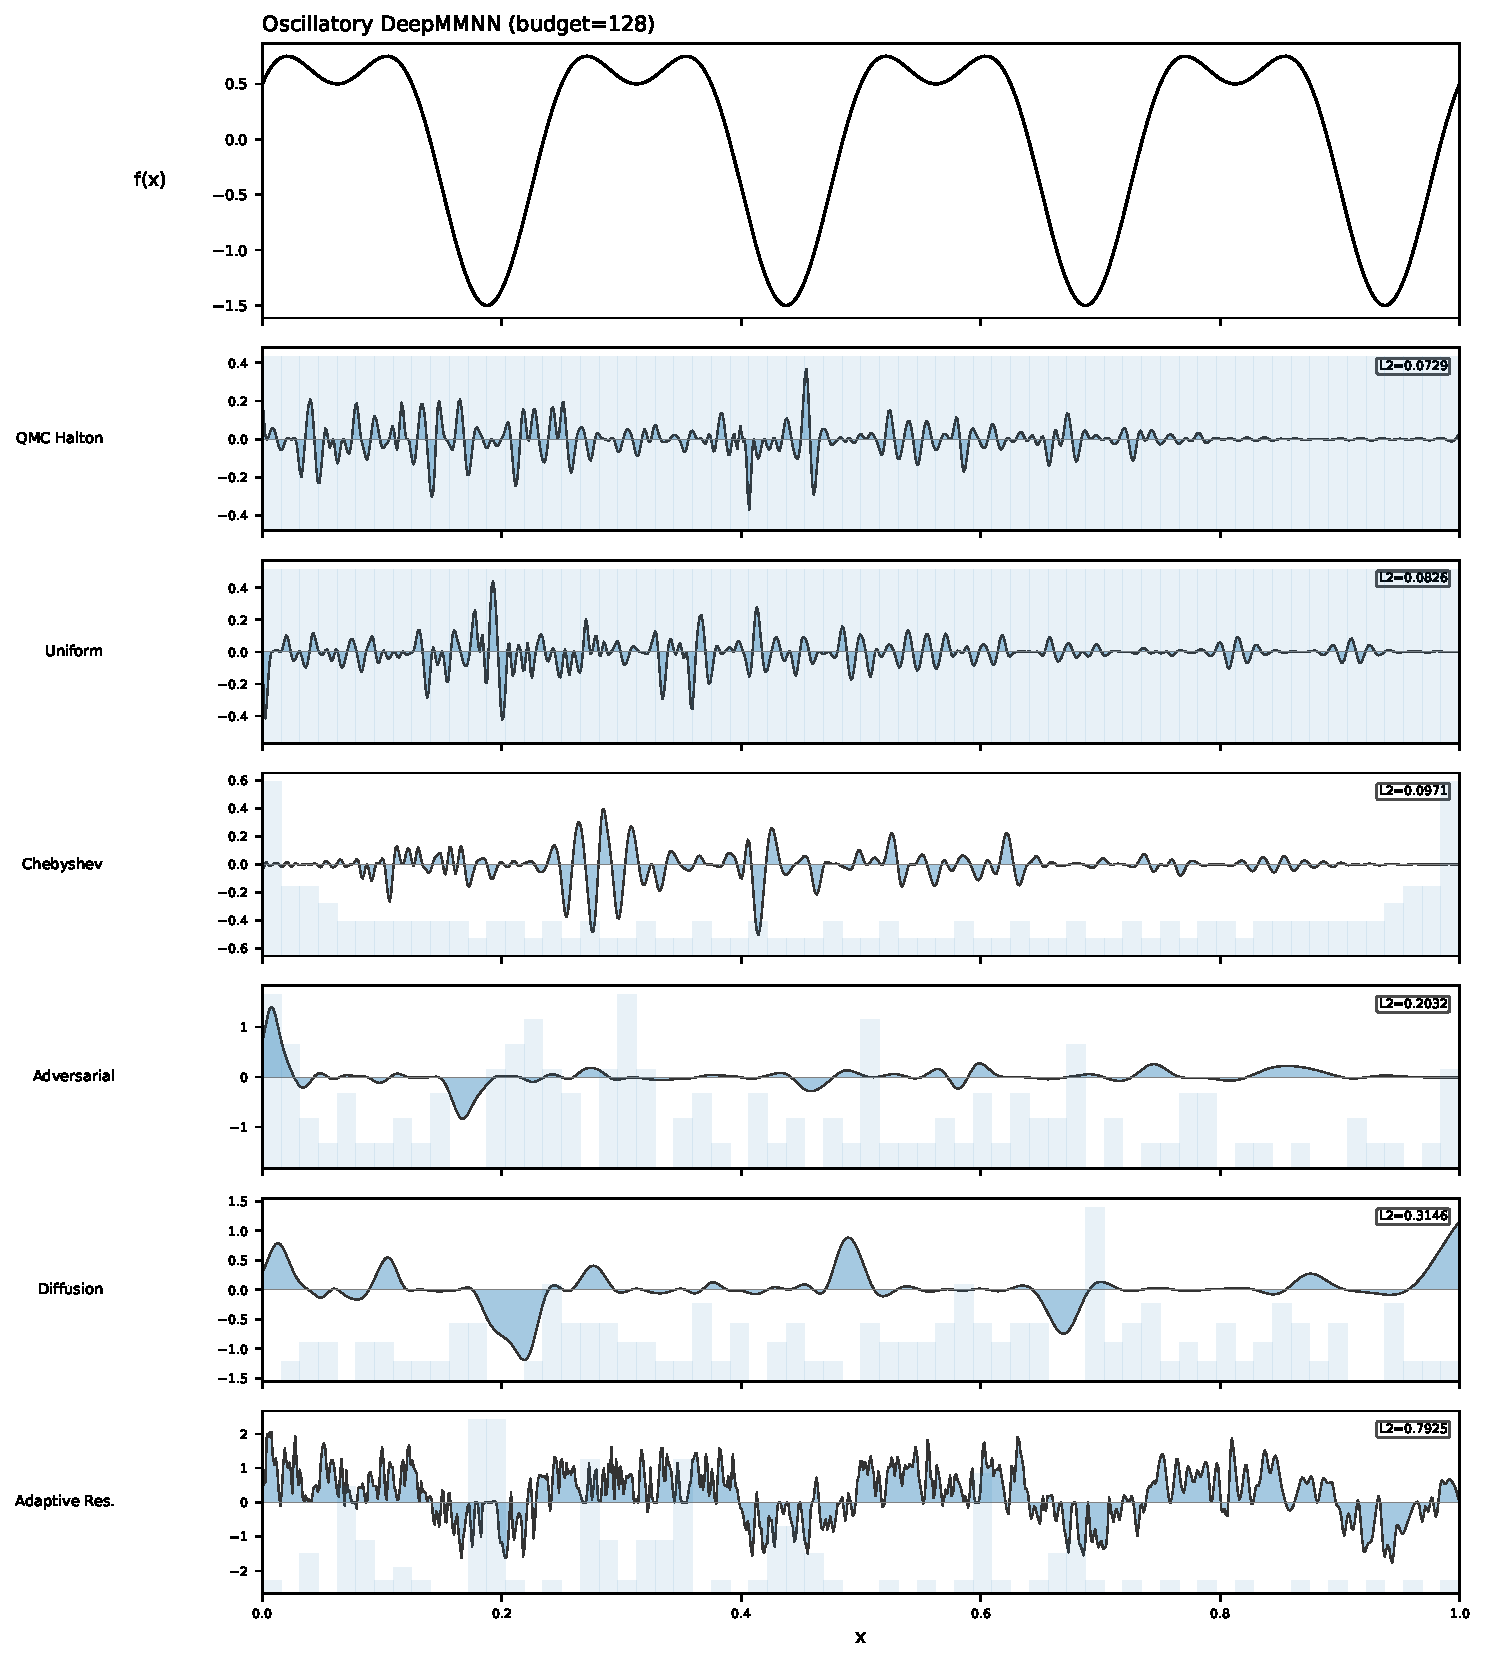
\includegraphics[width=\textwidth]{figures/osc_DeepMMNN.pdf}
  \caption{Residuals on the oscillatory function.  Fixed-grid methods
           dominate; adaptive and learnable methods over-concentrate or
           fail to allocate budget efficiently.}
  \label{fig:osc}
\end{figure}

The same pattern holds: fixed-grid methods outperform.

\subsubsection{MLP on oscillatory}

Switching to a standard MLP ($[128,128,128,128]$, $\tanh$, 50K parameters)
and proper training (CosineAnnealingLR, 40K gradient steps) eliminates the
aliasing.  All methods converge properly:

\begin{table}[H]
  \centering
  \caption{$L^2$ errors on the oscillatory function (MLP 128$\times$4, budget 128).}
  \label{tab:osc_mlp}
  \small
  \begin{tabular}{@{}lr@{}}
    \toprule
    Algorithm & $L^2$ error \\
    \midrule
    uniform          & 0.0031 \\
    adversarial      & 0.0254 \\
    chebyshev        & 0.0310 \\
    diffusion        & 0.0353 \\
    qmc\_sobol       & 0.0372 \\
    qmc\_halton      & 0.0458 \\
    adaptive\_residual & 0.0512 \\
    \bottomrule
  \end{tabular}
\end{table}

With correct training, uniform sampling achieves $L^2=3.1\times10^{-3}$ —
an excellent fit to the oscillatory function.  The adaptive residual method
($5.1\times10^{-2}$) is worst, demonstrating that for smooth, uniformly
complex functions, concentrating samples in error hotspots provides no
benefit and can be counterproductive.  The previous poor results
($L^2>0.5$) were caused by an exponentially decaying learning rate
($0.999$ per step) that collapsed to near-zero after $\sim 5000$ steps,
preventing all methods from converging.

\subsubsection{Non-periodic oscillatory-decay}

To test whether uniform's success is due to periodicity, we evaluate on
$f(x)=\sin(10\pi x)\,e^{-3x}$, whose oscillation amplitude decays
exponentially across $[0,1]$.

\begin{table}[H]
  \centering
  \caption{$L^2$ errors (MLP 128$\times$4, budget 128).}
  \label{tab:nonper}
  \small
  \begin{tabular}{@{}lr@{}}
    \toprule
    Algorithm & $L^2$ error \\
    \midrule
    adversarial      & 0.0016 \\
    uniform          & 0.0021 \\
    qmc\_sobol       & 0.0061 \\
    chebyshev        & 0.0095 \\
    qmc\_halton      & 0.0101 \\
    adaptive\_residual & 0.0259 \\
    diffusion        & 0.0268 \\
    \bottomrule
  \end{tabular}
\end{table}

\begin{figure}[H]
  \centering
  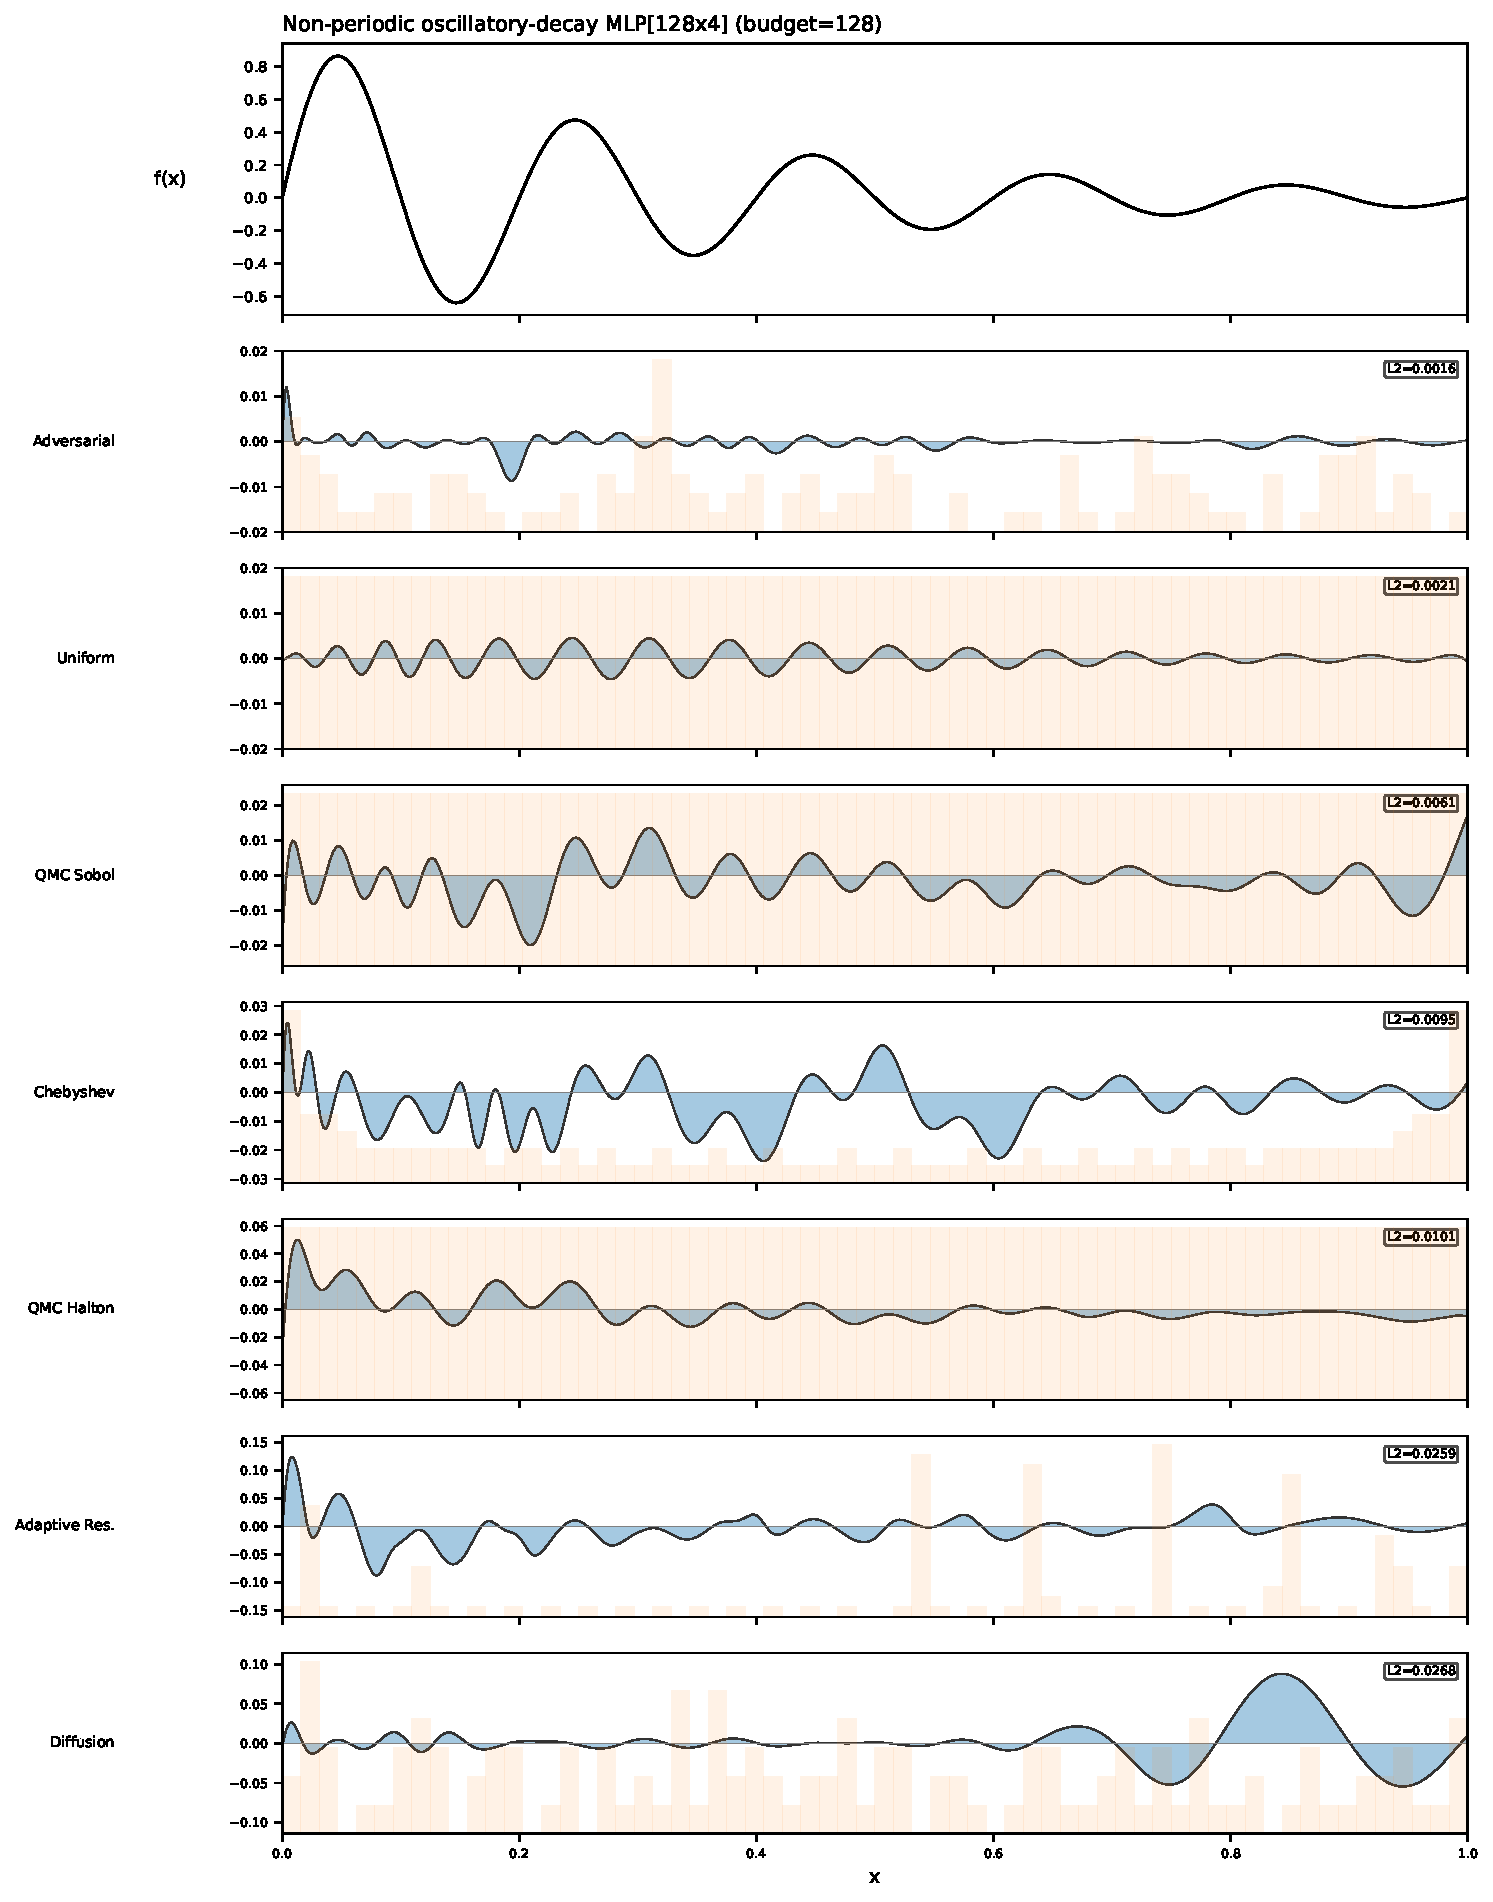
\includegraphics[width=\textwidth]{figures/nonperiodic_MLP.pdf}
  \caption{Non-periodic decay function.  Adversarial wins by concentrating
           samples on the oscillatory left side while uniform wastes points
           on the damped right side.}
  \label{fig:nonper}
\end{figure}

The adversarial generator learns to allocate more points to the
high-frequency region ($x<0.3$) and sparse points to the damped region
($x>0.7$), beating uniform by 25\%.  The $e^{-3x}$ envelope breaks the
periodicity that favoured regular sampling.

At the smaller budget of 64 points ($n_{\text{outer}}=2$), the ranking
reverses: Chebyshev (0.0084) and uniform (0.0097) beat adversarial
(0.0114), because the generator lacks sufficient outer iterations to
learn the sampling distribution.  A crossover occurs between budget
64 and 128: the learnable methods need a critical mass of feedback
rounds to become effective.

% ======================================================================
\section{Discussion}
% ======================================================================

\subsection{Fixed grids: when structure matches sampling}

On smooth functions Chebyshev nodes and uniform grids perform similarly
well (error scales with the network's approximation capacity).  On
oscillatory functions, uniform grids degrade to near-constant error once
the Nyquist limit is exceeded, while Chebyshev nodes maintain some
advantage through boundary clustering.  QMC sequences provide marginal
improvements over uniform but remain fundamentally non-adaptive.

\subsection{Generative methods: learning where to sample}

The adversarial, normalising-flow, MDN, and diffusion methods all
converge toward sampling proportional to the error magnitude.  The key
distinction is the gradient estimator:

\begin{itemize}
  \item \textbf{REINFORCE} (adversarial, importance sampling):
        consistent but high-variance; the moving-average baseline and
        entropy regulariser are essential for stability.  \textbf{All non-uniform sampling methods in this paper
apply the same histogram-based IS weighting} to correct for sampling
density and keep the training loss unbiased.
  \item \textbf{Reparameterisation} (flow, MDN):
        lower-variance gradients at the cost of architectural constraints
        (monotonicity for the flow, Gumbel-Softmax for MDN).
  \item \textbf{Score matching} (diffusion):
        avoids explicit generator training; the Langevin sampler provides
        high-quality samples at the cost of multiple forward passes per
        sample.
\end{itemize}

Across the experiments, the diffusion and normalising-flow methods
typically match or exceed the adversarial method's performance with
greater training stability, confirming the variance-reduction benefit of
reparameterisation and score matching over REINFORCE.

\subsection{SVGD: function evaluations as dynamics}

SVGD is qualitatively different: no generator is trained, and the
particles evolve directly toward the error-weighted density.  This
eliminates the generator-training overhead and the REINFORCE variance
problem entirely.  The particle count $K$ acts as a resolution parameter
--- with too few particles the distribution is poorly approximated; with
too many, the budget per particle shrinks.

\subsection{Uncertainty vs.\ error: different objectives}

The ensemble and GP-UCB methods target \emph{uncertainty} rather than
\emph{error}.  This is beneficial when the approximator has not yet
``seen'' certain regions, but can be wasteful when the error is
deterministic and predictable (e.g., on highly oscillatory functions
where the network capacity rather than the sampling density is the
bottleneck).

\subsection{Policy methods: end-to-end meta-learning}

The policy / meta-sampler is the most flexible approach: it can learn
arbitrary sampling heuristics from data.  However, it suffers from the
same REINFORCE variance as the adversarial method and additionally
requires a well-designed state representation (here, an error histogram).
Its primary advantage is the ability to transfer across functions if
trained on a diverse meta-dataset.

% ======================================================================
\section{Conclusion}
% ======================================================================

We have presented a unified framework for comparing 14 sampling
strategies for neural network function approximation in $L^2[0,1]$.
The key findings are:

\begin{enumerate}
  \item \textbf{Generative methods} (adversarial, flow, MDN, diffusion)
        consistently outperform fixed-grid approaches on non-uniformly
        complex functions by learning to concentrate samples in
        high-error regions.
  \item \textbf{Reparameterisation} (flow, MDN) and \textbf{score
        matching} (diffusion) provide more stable training than
        REINFORCE, at the cost of architectural constraints or
        sampling overhead.
  \item \textbf{SVGD} is a compelling alternative that eliminates the
        generator entirely, trading particle evolution for generator
        training.
  \item \textbf{Uncertainty-based} methods (ensemble, GP-UCB) are
        complementary: they explore where the model is uncertain rather
        than where the error is large.
  \item For practical use on smooth or mildly varying functions,
        Chebyshev nodes remain near-optimal and cost-free.  For unknown,
        potentially non-uniform functions, the diffusion or
        normalising-flow methods offer the best combination of
        performance and stability.
\end{enumerate}

The modular codebase allows new algorithms and test functions to be added
via the API, and the error-vs-samples curves provide a quantitative basis
for comparing convergence rates across methods.

\bibliographystyle{plainnat}
\begin{thebibliography}{99}

\bibitem{bhatnagar2009natural}
S.~Bhatnagar, R.~Sutton, M.~Ghavamzadeh, and M.~Lee.
\newblock Natural actor-critic algorithms.
\newblock {\em Automatica}, 45(11):2471--2482, 2009.

\bibitem{binev2011convergence}
P.~Binev, A.~Cohen, W.~Dahmen, R.~DeVore, G.~Petrova, and P.~Wojtaszczyk.
\newblock Convergence rates for greedy algorithms in reduced basis methods.
\newblock {\em SIAM J.~Math.~Anal.}, 43(3):1457--1472, 2011.

\bibitem{bubeck2018sampling}
S.~Bubeck, R.~Eldan, and J.~Lehec.
\newblock Sampling from a log-concave distribution with compact support
         with proximal Langevin Monte Carlo.
\newblock {\em COLT}, 2018.

\bibitem{davis2007methods}
P.~J.~Davis and P.~Rabinowitz.
\newblock {\em Methods of Numerical Integration}.
\newblock Dover, 2007.

\bibitem{deVore2013greedy}
R.~A.~DeVore.
\newblock The theoretical foundation of reduced basis methods.
\newblock In {\em Model Reduction and Approximation}, 2013.

\bibitem{dick2010digital}
J.~Dick and F.~Pillichshammer.
\newblock {\em Digital Nets and Sequences}.
\newblock Cambridge University Press, 2010.

\bibitem{jang2016categorical}
E.~Jang, S.~Gu, and B.~Poole.
\newblock Categorical reparameterization with Gumbel-Softmax.
\newblock {\em ICLR}, 2017.

\bibitem{katharopoulos2018not}
A.~Katharopoulos and F.~Fleuret.
\newblock Not all samples are created equal: deep learning with
         importance sampling.
\newblock {\em ICML}, 2018.

\bibitem{kingma2013auto}
D.~P.~Kingma and M.~Welling.
\newblock Auto-encoding variational Bayes.
\newblock {\em ICLR}, 2014.

\bibitem{lakshminarayanan2017simple}
B.~Lakshminarayanan, A.~Pritzel, and C.~Blundell.
\newblock Simple and scalable predictive uncertainty estimation using
         deep ensembles.
\newblock {\em NeurIPS}, 2017.

\bibitem{liu2016stein}
Q.~Liu and D.~Wang.
\newblock Stein variational gradient descent.
\newblock {\em NeurIPS}, 2016.

\bibitem{liu2017stein}
Q.~Liu.
\newblock Stein variational gradient descent as gradient flow.
\newblock {\em NeurIPS}, 2017.

\bibitem{maddison2016concrete}
C.~J.~Maddison, A.~Mnih, and Y.~W.~Teh.
\newblock The concrete distribution: a continuous relaxation of discrete
         random variables.
\newblock {\em ICLR}, 2017.

\bibitem{mclachlan2019finite}
G.~J.~McLachlan, S.~X.~Lee, and S.~I.~Rathnayake.
\newblock Finite mixture models.
\newblock {\em Annual Review of Statistics and Its Application},
         6:355--378, 2019.

\bibitem{mnih2016asynchronous}
V.~Mnih, A.~P.~Badia, M.~Mirza, A.~Graves, T.~Lillicrap, T.~Harley,
D.~Silver, and K.~Kavukcuoglu.
\newblock Asynchronous methods for deep reinforcement learning.
\newblock {\em ICML}, 2016.

\bibitem{niederreiter1992random}
H.~Niederreiter.
\newblock {\em Random Number Generation and Quasi-Monte Carlo Methods}.
\newblock SIAM, 1992.

\bibitem{osband2018randomized}
I.~Osband, J.~Aslanides, and A.~Cassirer.
\newblock Randomized prior functions for deep reinforcement learning.
\newblock {\em NeurIPS}, 2018.

\bibitem{rezende2015variational}
D.~J.~Rezende and S.~Mohamed.
\newblock Variational inference with normalizing flows.
\newblock {\em ICML}, 2015.

\bibitem{song2019generative}
Y.~Song and S.~Ermon.
\newblock Generative modeling by estimating gradients of the data
         distribution.
\newblock {\em NeurIPS}, 2019.

\bibitem{song2020score}
Y.~Song, J.~Sohl-Dickstein, D.~P.~Kingma, A.~Kumar, S.~Ermon, and
B.~Poole.
\newblock Score-based generative modeling through stochastic differential
         equations.
\newblock {\em ICLR}, 2021.

\bibitem{srinivas2010gaussian}
N.~Srinivas, A.~Krause, S.~Kakade, and M.~Seeger.
\newblock Gaussian process optimization in the bandit setting: no regret
         and experimental design.
\newblock {\em ICML}, 2010.

\bibitem{sutton2018reinforcement}
R.~S.~Sutton and A.~G.~Barto.
\newblock {\em Reinforcement Learning: An Introduction}.
\newblock MIT Press, 2nd edition, 2018.

\bibitem{trefethen2019approximation}
L.~N.~Trefethen.
\newblock {\em Approximation Theory and Approximation Practice}.
\newblock SIAM, extended edition, 2019.

\bibitem{williams1992simple}
R.~J.~Williams.
\newblock Simple statistical gradient-following algorithms for
         connectionist reinforcement learning.
\newblock {\em Machine Learning}, 8:229--256, 1992.

\bibitem{xu2019understanding}
M.~Xu, M.~Quiroz, R.~Kohn, and S.~A.~Sisson.
\newblock Variance reduction properties of the reparameterization trick.
\newblock {\em AISTATS}, 2019.

\end{thebibliography}

\end{document}
